\documentclass[oneside,a4paper,11pt,explicit]{book}
\usepackage[utf8]{inputenc}
\usepackage{icecream}
\usepackage[english]{babel}
\addto\captionsenglish{\renewcommand{\chaptername}{}}
\usepackage[accsupp]{axessibility}  % improves PDF readability for those with disabilities.
\usepackage[colorlinks = true,urlcolor  = blue,linkcolor = blue]{hyperref}
\usepackage{setspace}
\usepackage{listings}
\usepackage[most]{tcolorbox}
\usepackage{minitoc}


\renewcommand{\mtifont}{\large\sffamily}
\renewcommand{\mtcfont}{\small\sffamily}
\renewcommand{\mtcSfont}{\small\sffamily}
\renewcommand{\mtcSSfont}{\small\sffamily}
\renewcommand{\mtcSSSfont}{\small\sffamily}
\mtcsetpagenumbers{minitoc}{off} % turn off page numbering in minitocs
\addto{\captionsenglish}{% Making babel aware of special titles
	\renewcommand{\mtctitle}{Quick Links To Sections}
}
\setlength{\fboxrule}{5pt}
\setlength{\fboxsep}{4pt}

\definecolor{IceCreamLeaf}{rgb}{0.4, 0.639215686274, 0.4}
\definecolor{IceCreamOrbit}{rgb}{0.803921568627451, 0.3607843137254902, 0.3607843137254902}

\title{I.C.E.C.R.E.A.M. Tutorials}
\subtitle{\small Observing Earth from Above (Env 329) - Fall 2023  \\
	\small Schmid College of Science and Technology, Chapman University}
\date{\today}

%% DOCUMENT
\setstretch{1.25}
\makeatletter
\begin{document}

\dominitoc

%\tableofcontents

\setcounter{chapter}{4} %Insert (Tutorial Number-1) Here; example for tutorial 4, enter 3

\chapter{Adding Elements To Maps} %Enter Tutorial Name Here

\vspace{-2em}

\minitoc

\hrule

\vspace{1em}

\begin{tcolorbox}[enhanced,frame style image=blueshade.png,
	opacityback=0.75,opacitybacktitle=0.25,
	colback=blue!5!white,colframe=blue!75!black,title={\Large \textbf{Objectives:}}]
	\large
	\begin{enumerate}
		\item Learn the map making features in QGIS.
		\item Introduce basic map elements.
		\item Create a NASA worthy map of surface temperatures from Death Valley National Park.
		\item Combine all of your skills to make a map for your hometown showcasing the hottest and coldest temperatures for last year. 
	\end{enumerate}
\end{tcolorbox}

\clearpage

%%%%%%%%%%%%%%%%%%%%%%%%%%%%%%%%%% Change Header to Have a Smaller Logo for Remainder of the Document
\fancyhead{}
\fancyhead[C]{\begin{tikzpicture}[overlay, remember picture]
		\fill[Blue2] (current page.north west) rectangle ($(current page.north east)+(0,-1in)$);
		\node[anchor=north west, text=white, font=\Large, minimum size=1in, inner xsep=5mm, align=left] at (current page.north west) {\bf{\MakeUppercase{\@title}}\\\@subtitle};
		\node[anchor=north east, minimum size=1in, inner xsep=5mm] at (current page.north east) {\includegraphics[scale=.125]{ICECREAM_Logo.png}};\end{tikzpicture}}
%%%%%%%%%%%%%%%%%%%%%%%%%%%%%%%%%%

\textbf{\underline{Motivation For Today's Tutorial : NASA Press Releases}}

\vspace{1 em}

{\centering

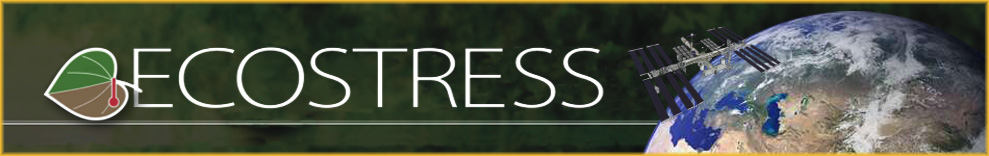
\includegraphics[width=\textwidth]{ecostress_banner.jpg}}

\vspace{1 em}

We want to begin to use satellite remote sensing data to understand environmental events as they happen and communicate them effectively with a broad audience. Today, we are going to create a  map of the Death Valley National Park surface temperatures similar to the last tutorial. However, today's tutorial will provide you with the basic working knowledge to create beautiful and informative maps. Later in the course, you will use these skills to analyze current environmental events and make your maps available to newsmedia and other public-facing outlets. 

\vspace{1 em}

\hrule

\section{Create A Base Map}

\centerline{\includegraphics[width=\textwidth]{Basemap.png}}

1. Create a new project (\textit{Project} $\rightarrow$ \textit{New})

\begin{singlespace}
2. Add the ESRI National Geographic Basemap by either:
	\begin{itemize}
		\item Using the \textit{XYZ Tiles} function in the \textit{Browser} window
		\item Using the \textit{HCMGIS} Menu (\textit{HCMGIS} $\rightarrow$ \textit{Basemaps} $\rightarrow$ \textit{ESRI National Geographic})
	\end{itemize}
\end{singlespace}

3. Zoom in to California.

4. Start a new print layout by going to the \textit{Project} menu, then select \textit{New Print Layout}. Enter whatever name you would like. I went with \textit{Death Valley Inset}.


\centerline{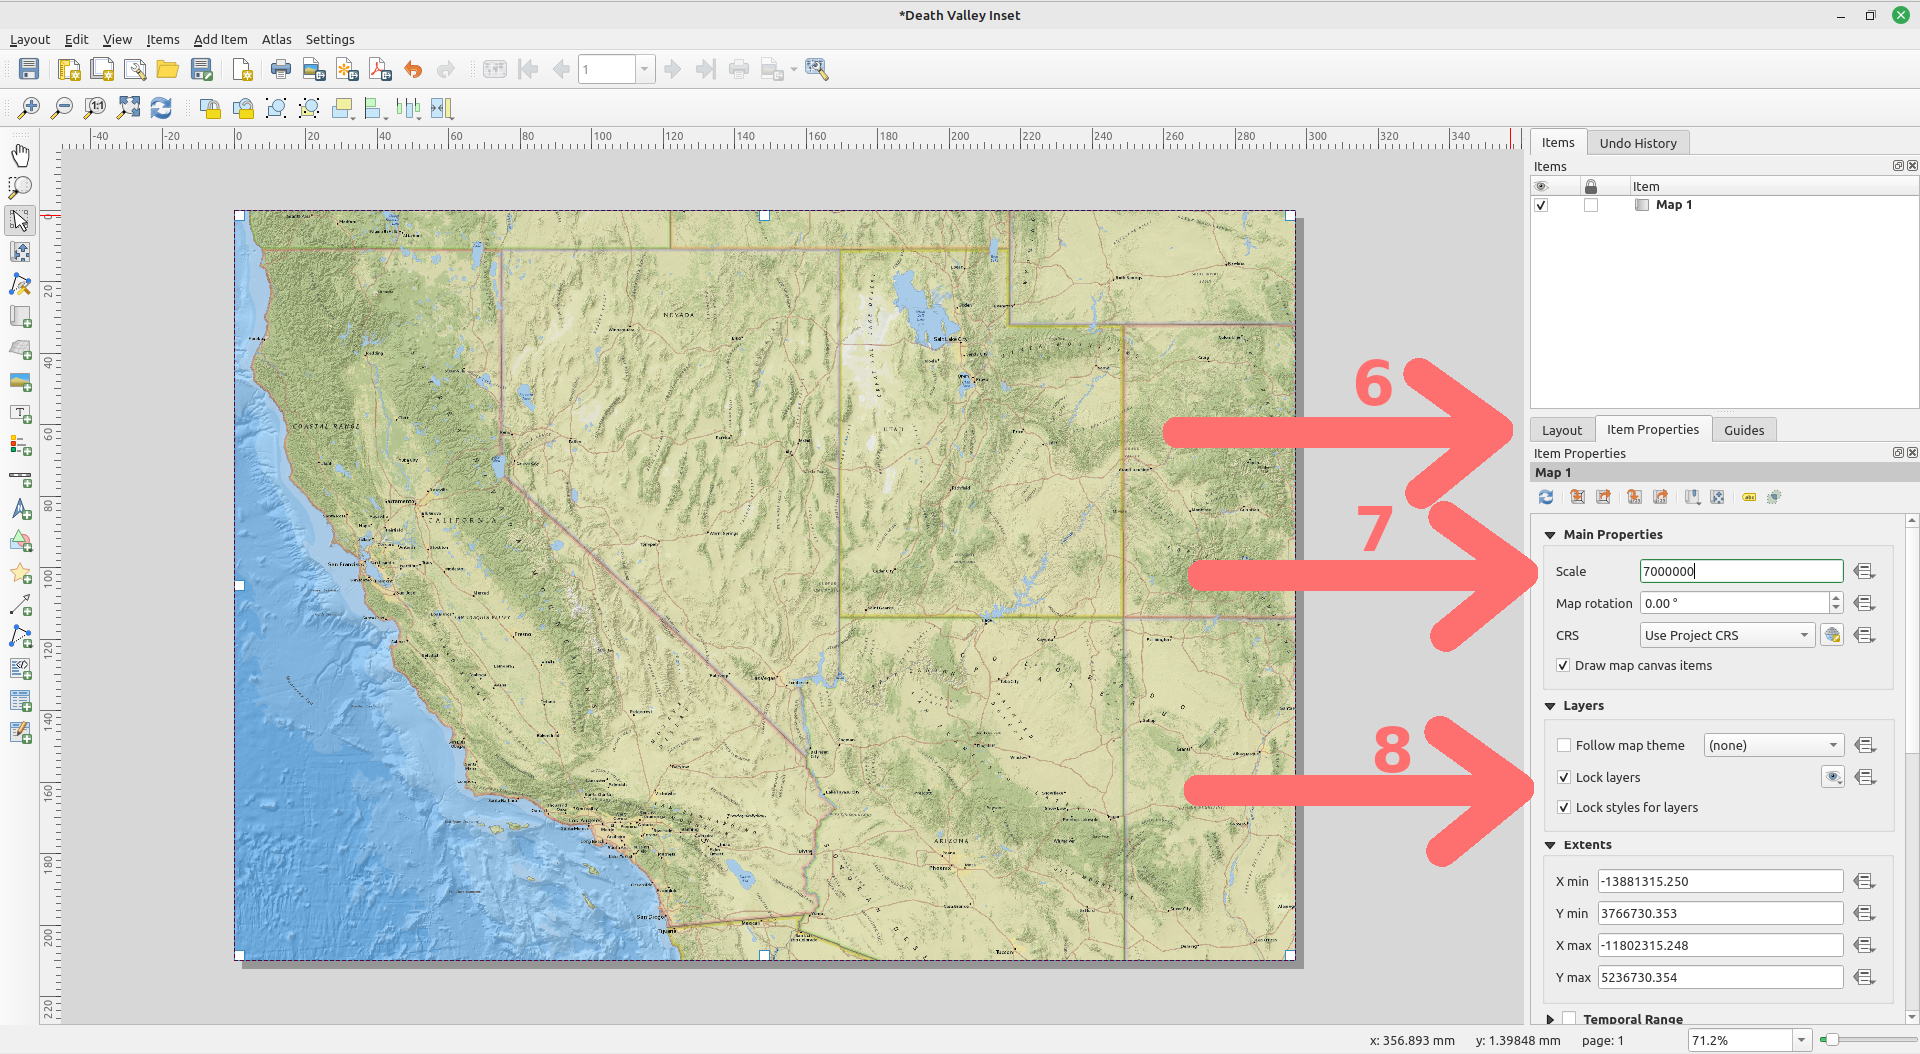
\includegraphics[width=\textwidth]{InsetItem.png}}

5. Now select the menu \textit{Add Item}, then \textit{Add Map}. Start at one corner of the white rectangle window and drag to the opposite diagonal corner to set the map space. You will see that the rectangle window will be rendered with the map from the main QGIS canvas.

6. Click on the \textit{Item Properties} tab.

7. Adjust the \textit{Scale}, which is the zoom level, to 7000000 and hit enter.

8. Check both \textit{Lock layers} and \textit{Lock layer styles} boxes. This will ensure that if we turn off some layers or change their styles, this view will not change.


\section{Add An Inset}

9. Let's add our map from the last tutorial as an inset to this map. First, return back to the main QGIS window. Add a second basemap layer following the same instructions as above, but this time use \textit{Google Satellite}.

10. Uncheck the box next to the ESRI National Geographic layer in the \emph{Layer} window, and QGIS will keep the layer in the project, but not display any of its information.

\subsection{Importing Our ECOSTRESS Death Valley Layer From The Previous Tutorial}
11. Use the \textit{browser} window to find the folder where you saved the two land surface temperature .tif files from the last tutorial. Double click each file to add them to your map.

12. Adjust the symbology for each of the land surface temperature layer by right clicking on the layer name in the \textit{Layers} window and select \textit{Layer Properties}. On the menu bar to the left select \textit{Symbology} and change the \textit{Render type} to Singleband pseudocolor. Use the red color ramp and remember to match the minimum and maximum values from the surface temperature: 306.82 as the minimum and 347 as the maximum for both layers. Click \textit{Apply}.

\centerline{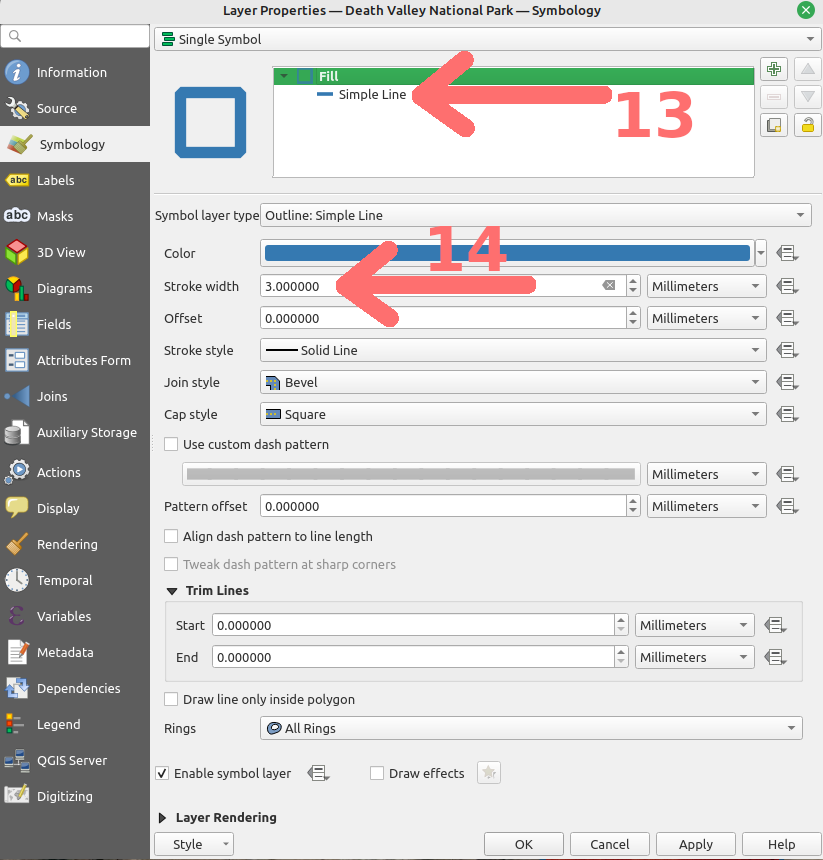
\includegraphics[width=.625\textwidth]{DVlines.png}}

13. Add in the border from the \textit{DeathValleyNationalPark.zip} shapefile. In the \textit{Browser} window, expand the zip file using the small arrow next to the filename. Double click on \textit{Death Valley National Park.shp} to add the layer. Right click on the layer in the \textit{Layers} window and change its symbology to \textit{outline blue}. 

14. The outline of the border is a little thin; let's make it thicker. First, click on the \textit{Simple Line} selection in the dialog box. Change the \textit{Stroke width} to 3 mm. Click the \textit{Apply} button at the bottom of the window.

15. Zoom in so that the outline of Death Valley National Park fits nicely in the window, it should look like this:

\vspace{.25em}

\centerline{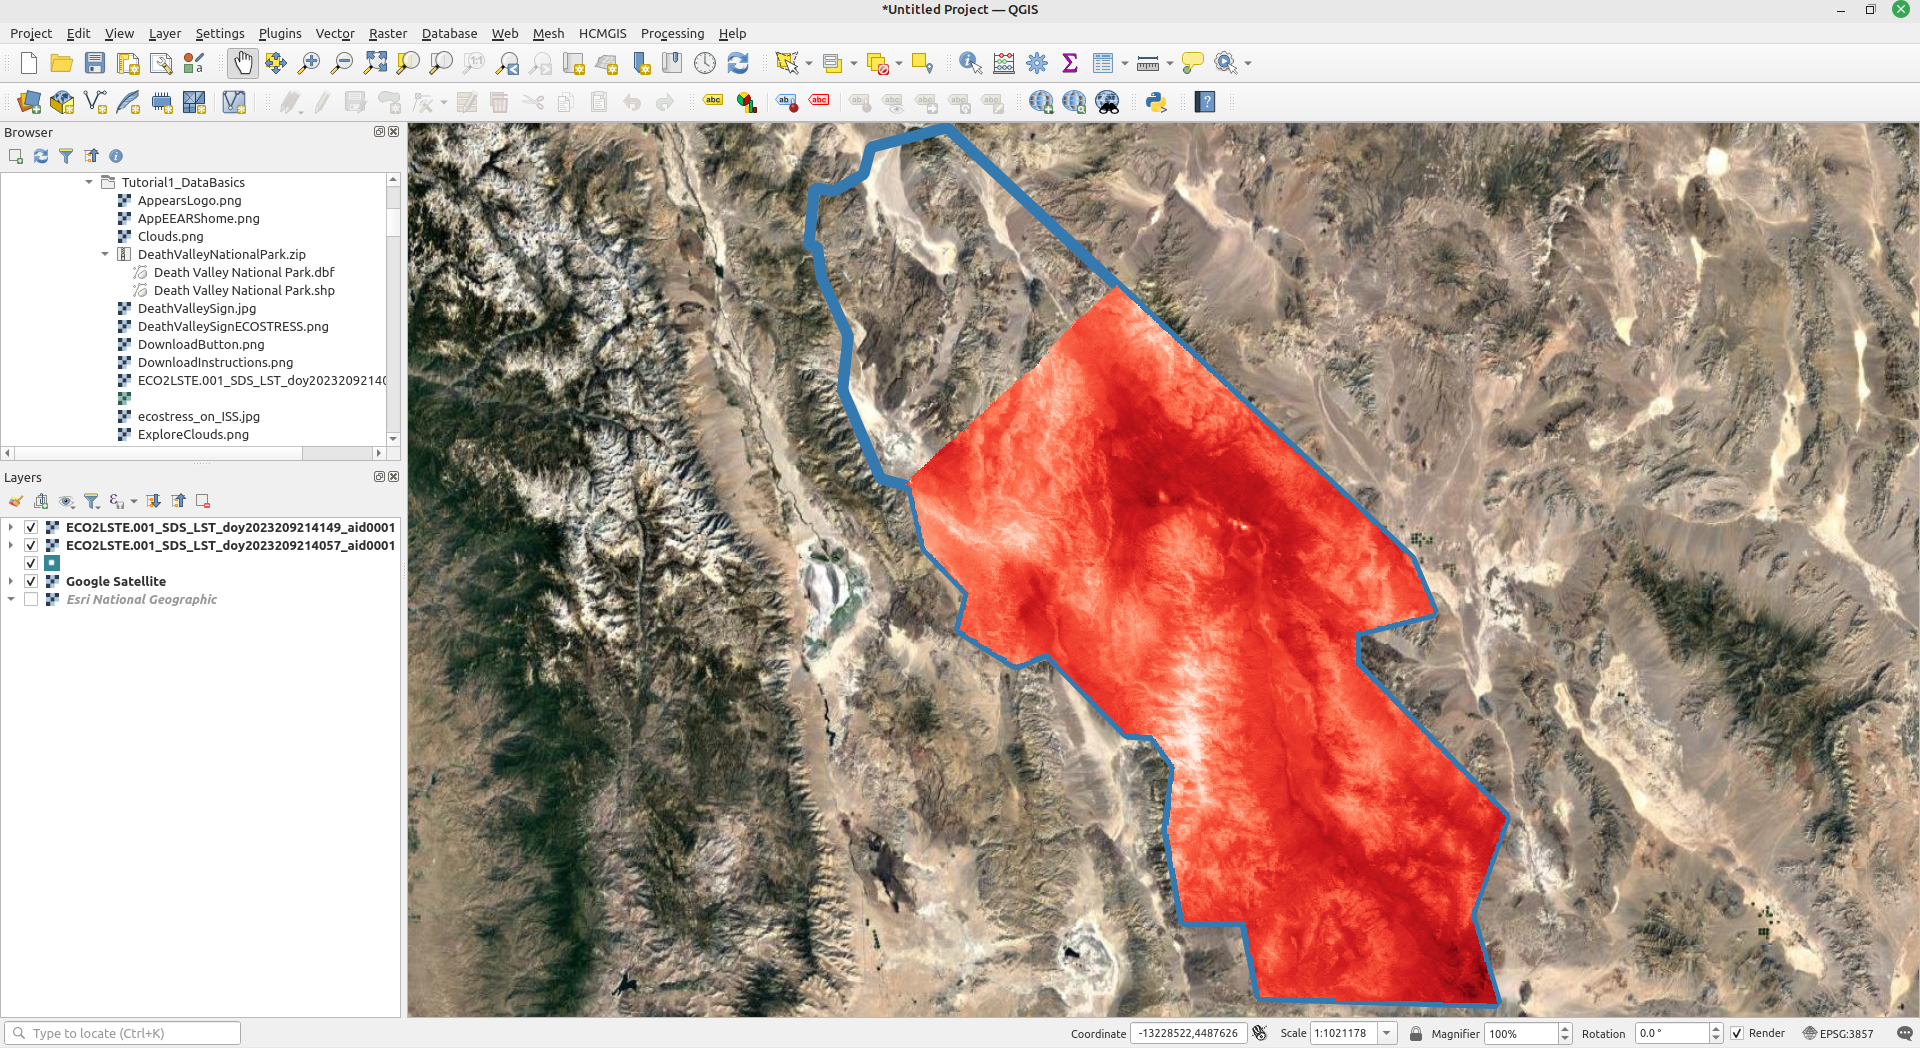
\includegraphics[width=\textwidth]{DV_LST.png}}

\subsection{Adding in our Land Surface Temperature Map as an Inset}

16. Now that we have the map how we like it the main window, switch back to the Print Layout window. Select the menu \textit{Add Item}, then \textit{Add Map}. Click and create an inset of the land surface temperature to the East of California.

\begin{tcolorbox}[enhanced jigsaw,breakable,pad at break*=1mm,
  colback=yellow!5!white,colframe=IceCreamLeaf,title=Inset Maps]
  An inset map is a smaller map within a larger map and can serve multiple purposes depending on your goals. Some things they can do:
    \begin{itemize}
         \item Provide context by showing the larger geographic region when the main map is zoomed in to a local scale:

         \vspace{.25em}
         
         \centerline{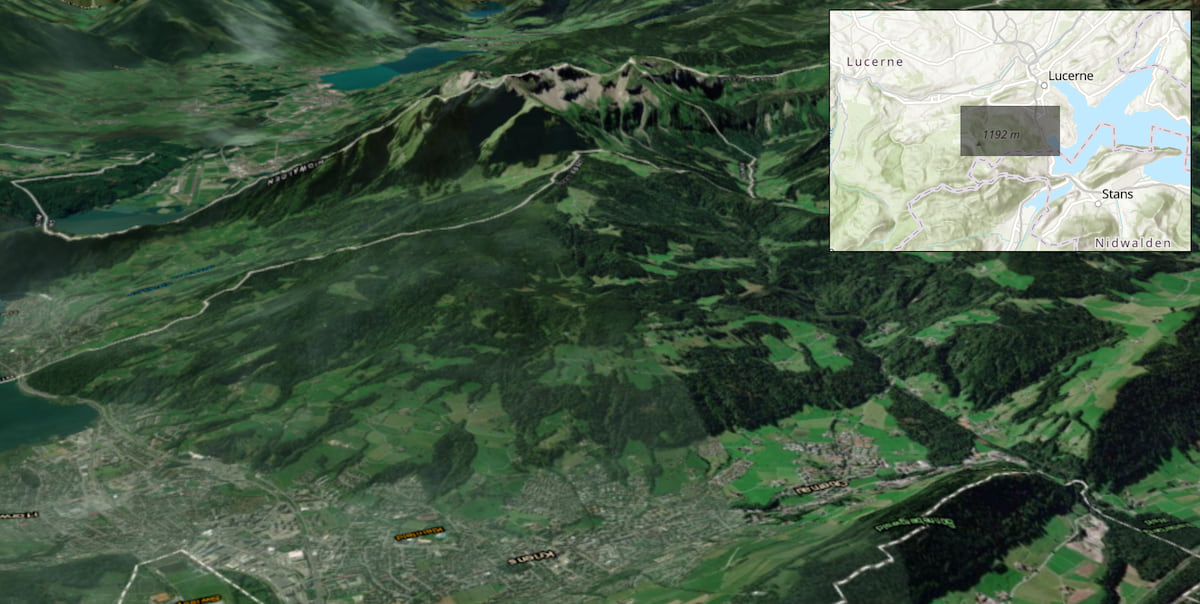
\includegraphics[width=.85\textwidth]{inset-overview.png}}

         \item Show more detail of a portion of the main map, when the main map is zoomed out to a broad scale:

         \vspace{.25em}
         
         \centerline{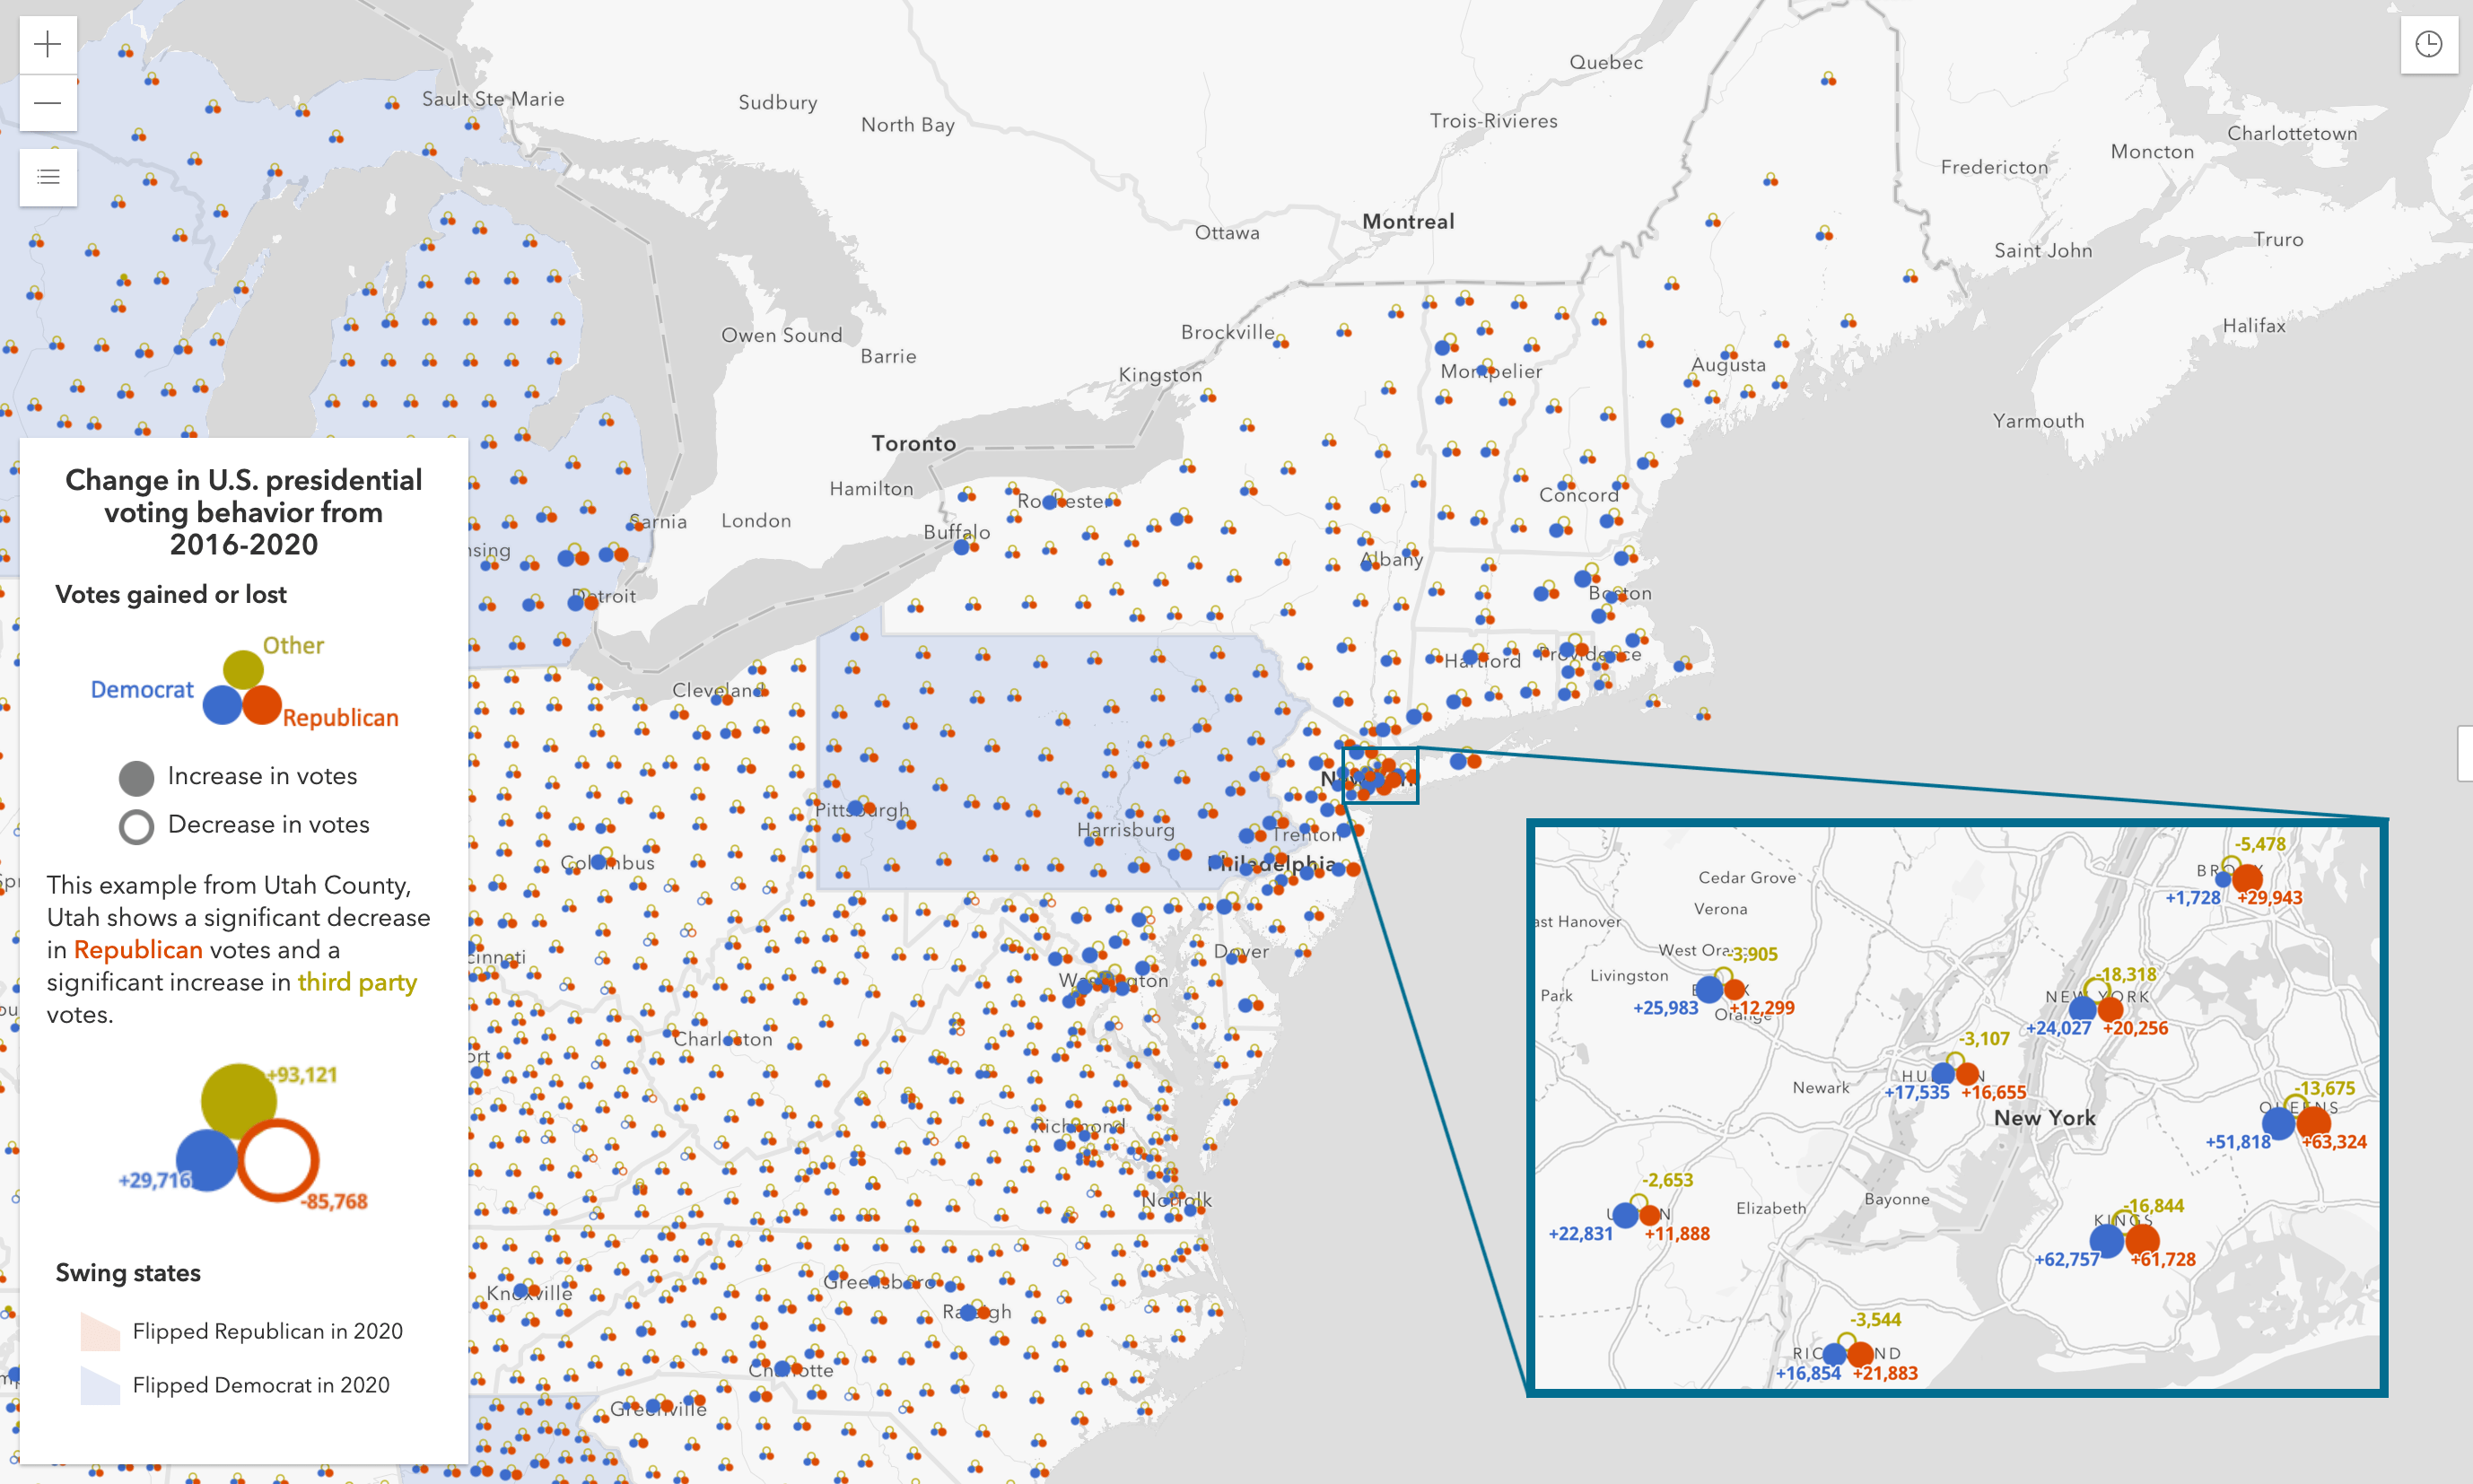
\includegraphics[width=.85\textwidth]{inset-detail.png}}

         \item Communicate additional data or information that complements the purpose of the main map area:

         \vspace{.25em}

         \centerline{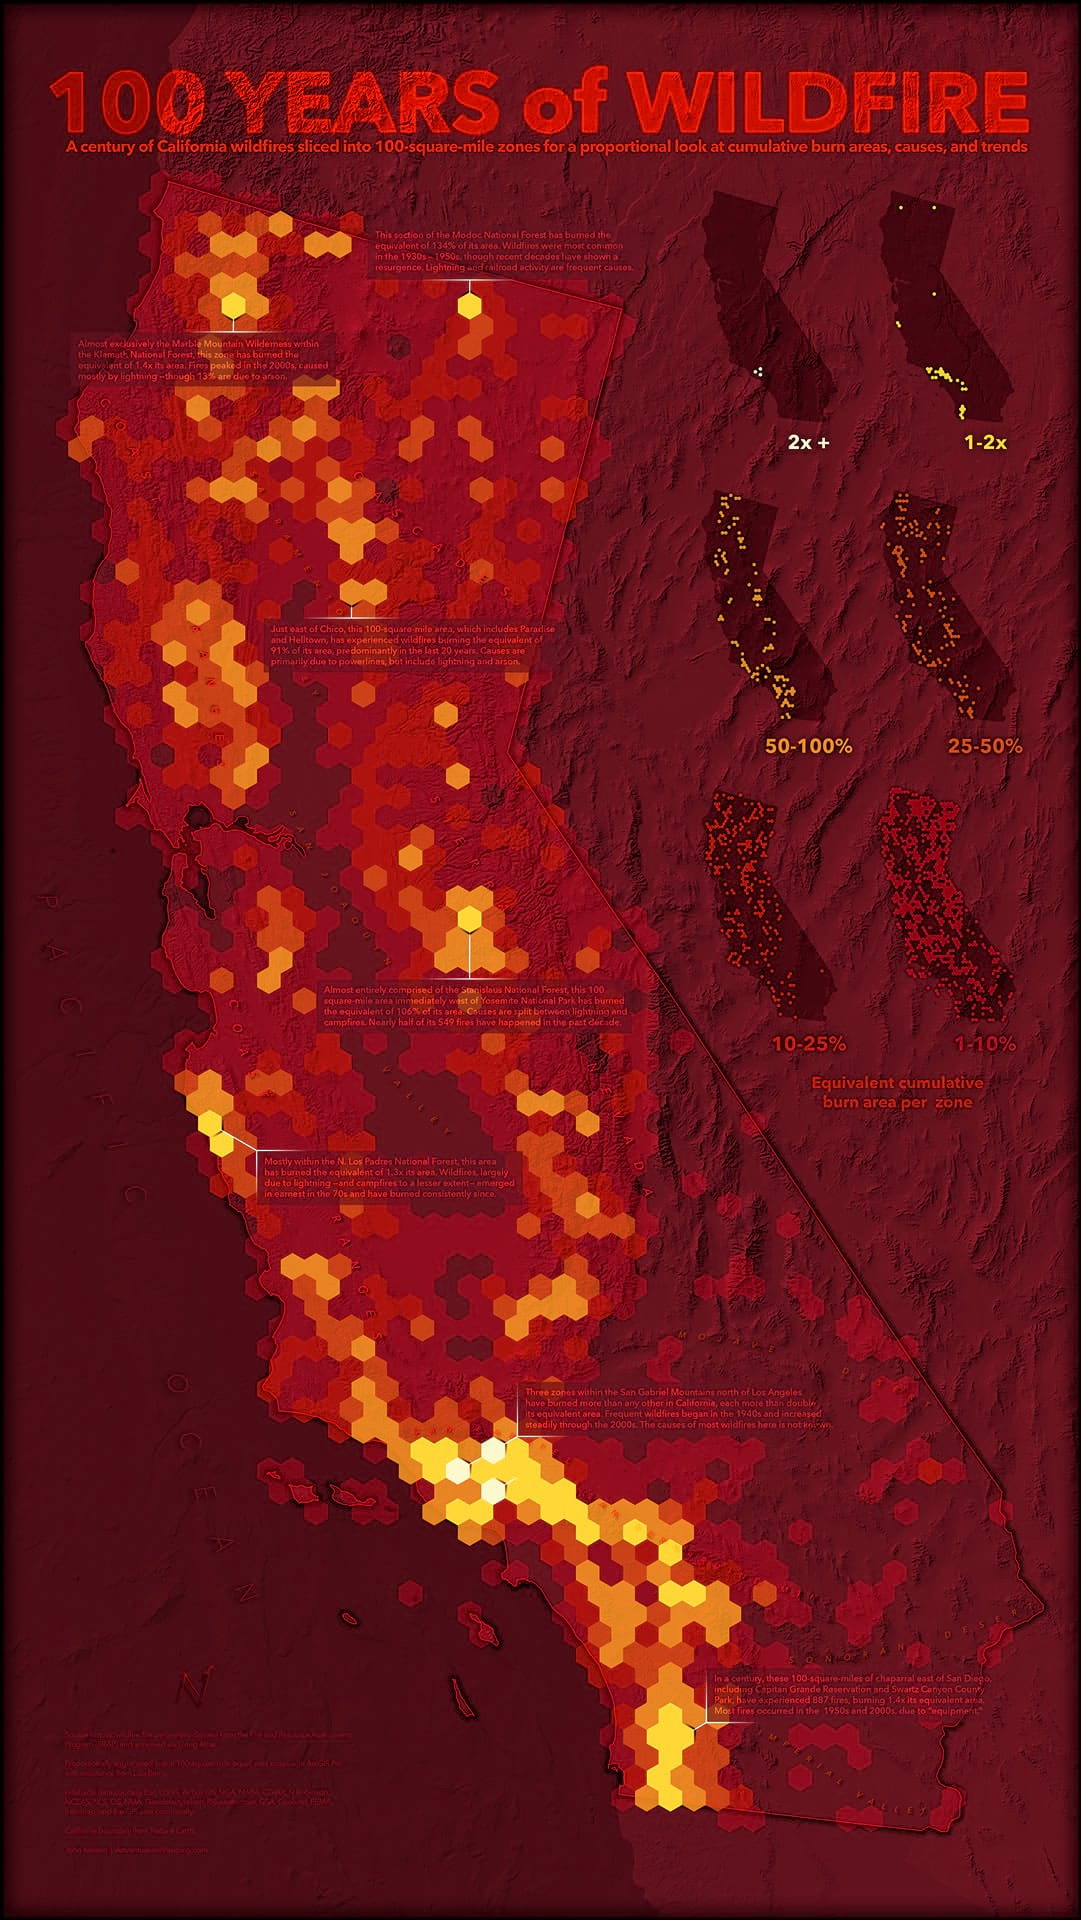
\includegraphics[width=.5\textwidth]{inset-multiples.jpg}}

         \item Display noncontiguous geometries at a single glance:

         \vspace{.25em}

         \centerline{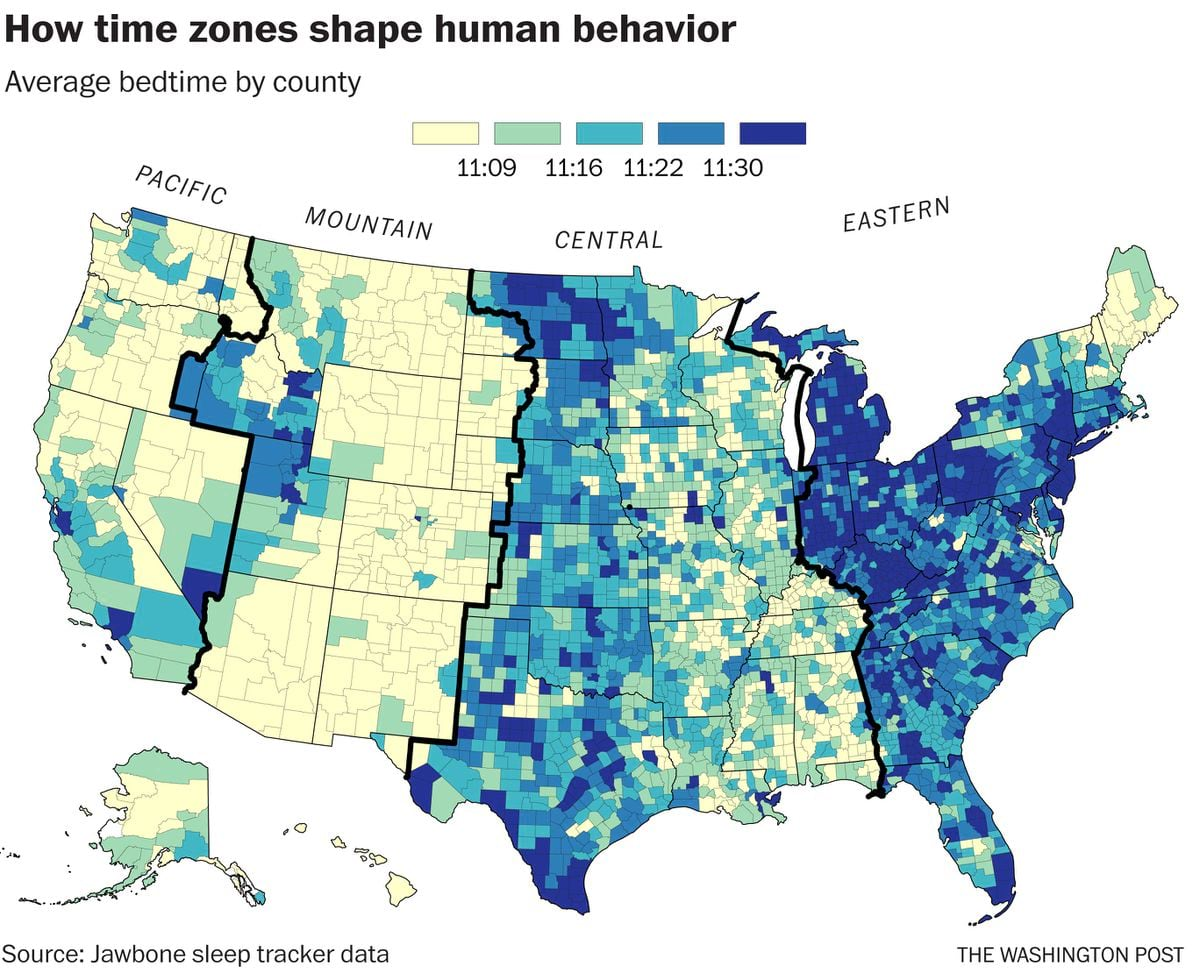
\includegraphics[width=.65\textwidth]{inset-noncontiguous.jpg}}
    \end{itemize}
\end{tcolorbox}



\vspace{.25em}

\centerline{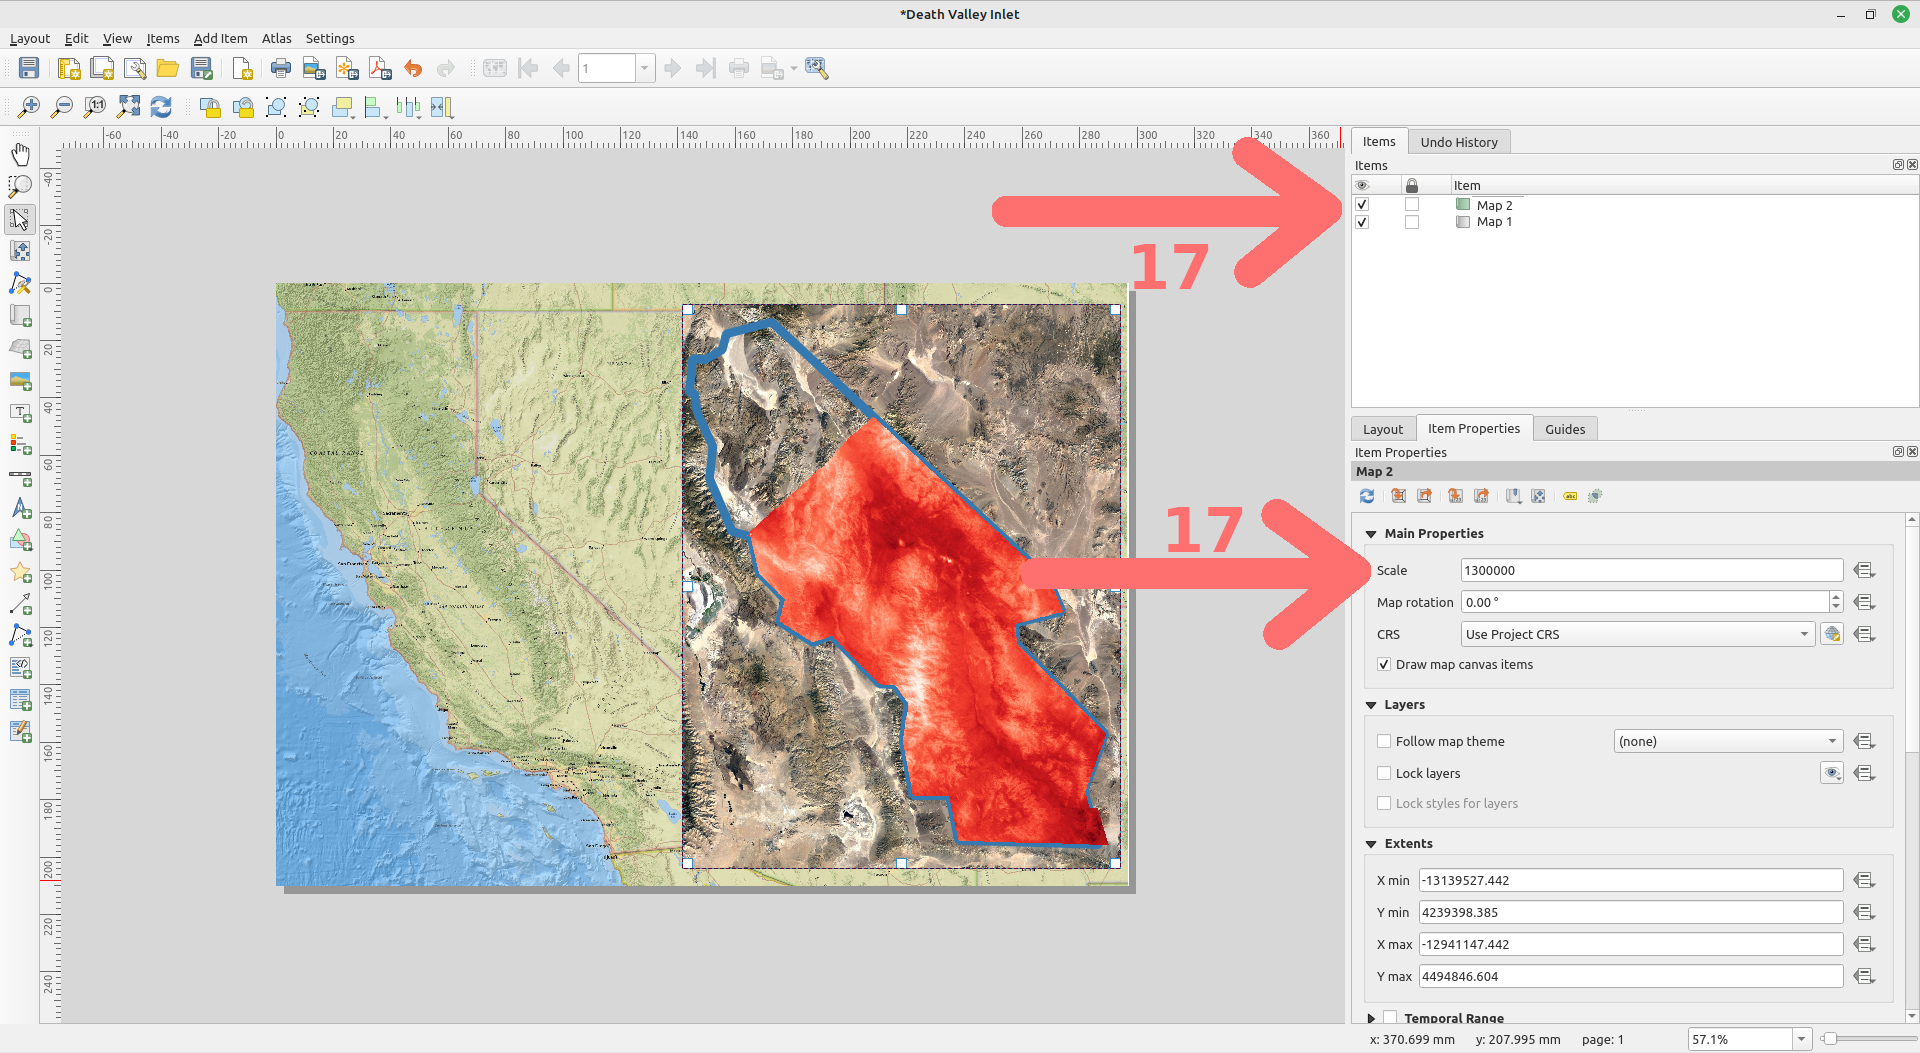
\includegraphics[width=\textwidth]{AddInset.png}}

17. Under the \textit{Item Properties} for the inset map (typically numbered \textit{Map 2} in the \textit{Items} window), change the scale to 1300000 to frame Death Valley. The scale is now fixed at 1:1300000 distance.

\vspace{.25em}

\centerline{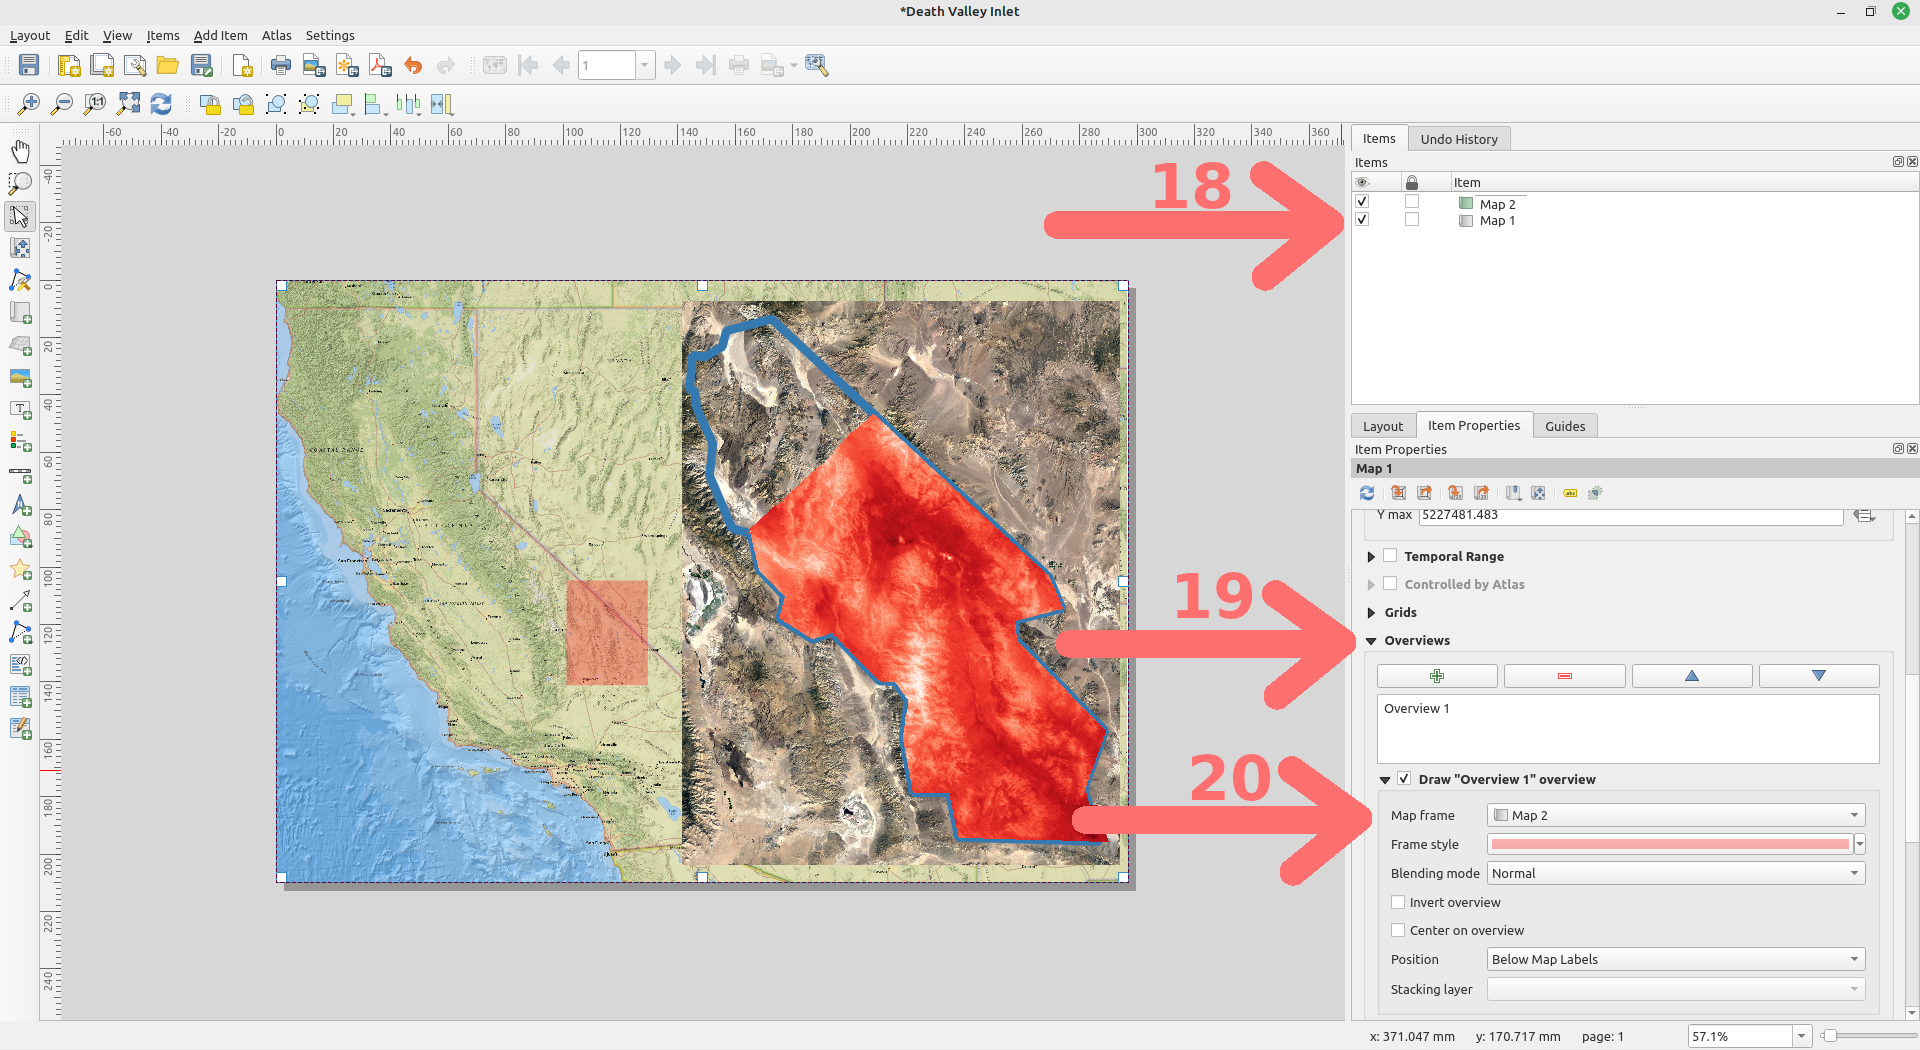
\includegraphics[width=\textwidth]{RegionShade.png}}

18. QGIS has an excellent tool for automatically highlighting the area on the main map that is represented in an inset. First, select \textit{Map 1} (or whatever your main map number is) in the \textit{Items} window.
 
19. Next, under \textit{Item Properties}, scroll down to find the \textit{Overviews} menu. Click the green plus sign to an overview.

20. Under map frame, select \textit{Map 2} (or whatever you have named your inset map). The area from the inset should now be highlighted on the main map. Adjust the highlight color to match your mood.

\section{Basic Map Elements}

\centerline{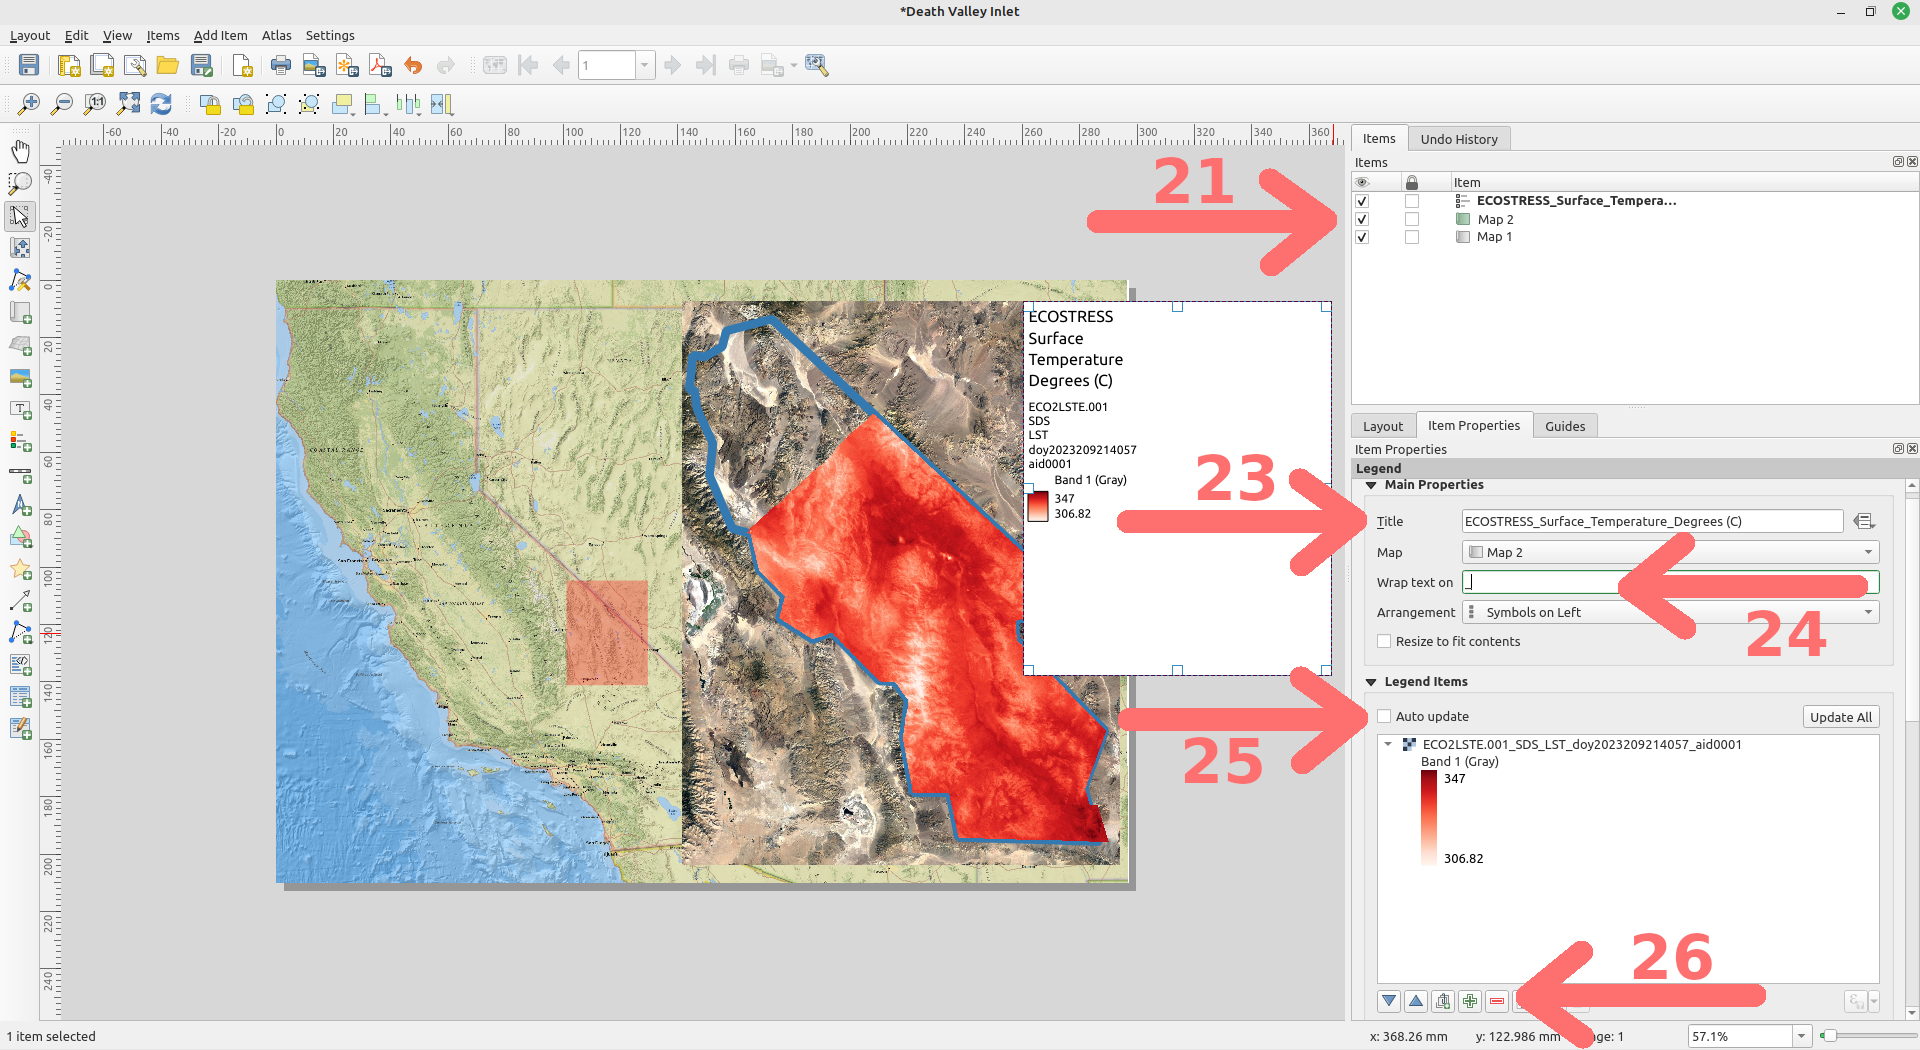
\includegraphics[width=\textwidth]{TempLegend1.png}}

\subsection{Adding a Legend}

A legend's function is to describe the visual information contained in a map, by explaining what the symbols and colors displayed on the map mean.

21. Select \textit{Map 2} from the \textit{Items} window.

22. From the \textit{Add Item} menu bar, select \textit{Legend}. Draw the legend as a box in the top left corner of the inset map. We can adjust its size later, so don't worry too much about how it looks right now.

23. Under \textit{Item Properties} enter ``ECOSTRESS\_Degrees (F)''. This will be the title of your legend. 

24. For \textit{Wrap text on} enter an underscore ``\_''. This will make the title of your legend split onto two lines at the underscore. 

25. Deselect the check box next to \textit{Auto update} to give us more control over what is displayed in the legend. Now we can customize it further.

26. We matched the temperature ranges for both of the layers, so only one legend entry is necessary. Remove all legend entries, except one of our ECOSTRESS surface temperature layers, by selecting the ones you want to remove and using the minus button. 

The SI unit of temperature set for the International System of Units is Kelvin (K), which is how the land surface temperature observations made by ECOSTRESS are reported. You can use the formulas below to convert K into degrees Celsius or Fahrenheit, which are often more intuitive to your target audiences. 
\begin{itemize}
	\item $C = K - 273.15$
	\item $F = (K - 273.15) \cdot \frac{9}{5} + 32$
\end{itemize}

\centerline{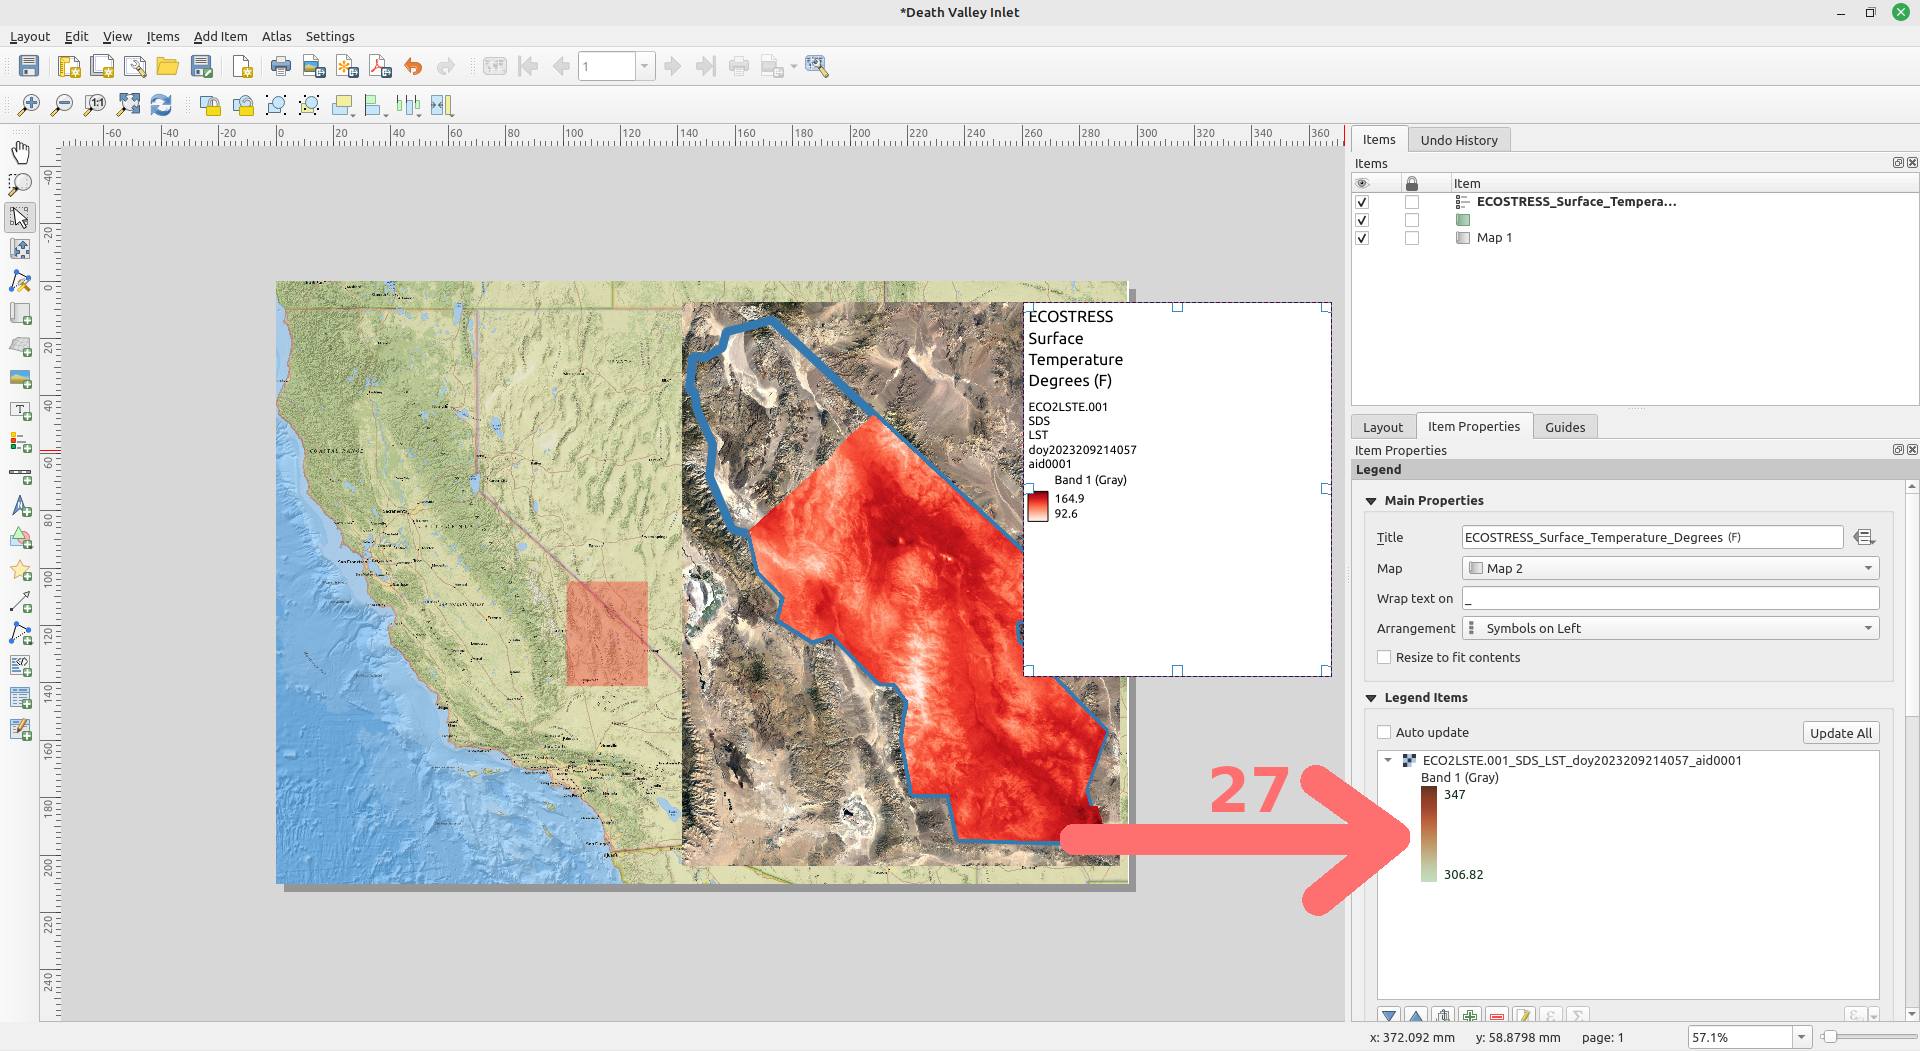
\includegraphics[width=\textwidth]{TempScale1.png}}

27. To change the scale of the legend bar, double click on the scale in the \textit{Legend Items} property window.

\vspace{.25em}

\centerline{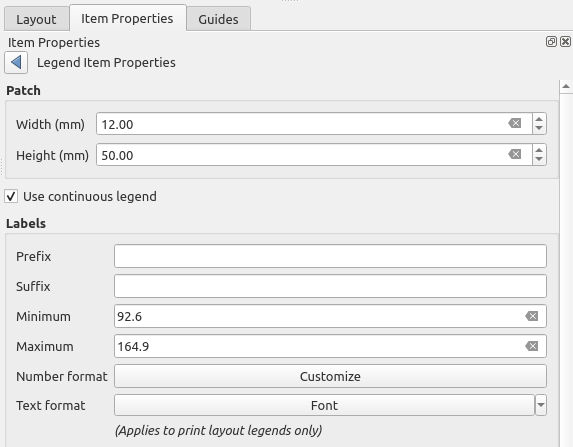
\includegraphics[width=.6\textwidth]{TempScale2.png}}

28. Converting our temperature scale to degrees Fahrenheit yields a range of 92.6 to 164.9, enter that range in the place of the default minimum and maximum values. Let's also adjust the width of the legend to 12 mm and the height to 60 mm. Use the back arrow to return to \textit{Item Properties}.

29. Let's make the legend look a little more professional by adjusting the background color. Scroll down and look for the \textit{Background} section of the \textit{Item Properties}. Use the arrow to expand your options. Here you can change the color, but for now let's leave it white but change the \textit{Opacity} to 44\%. This makes the legend back more transparent, giving it a cleaner look. It should resemble the screenshot above. Return back to the list of item properties.

\centerline{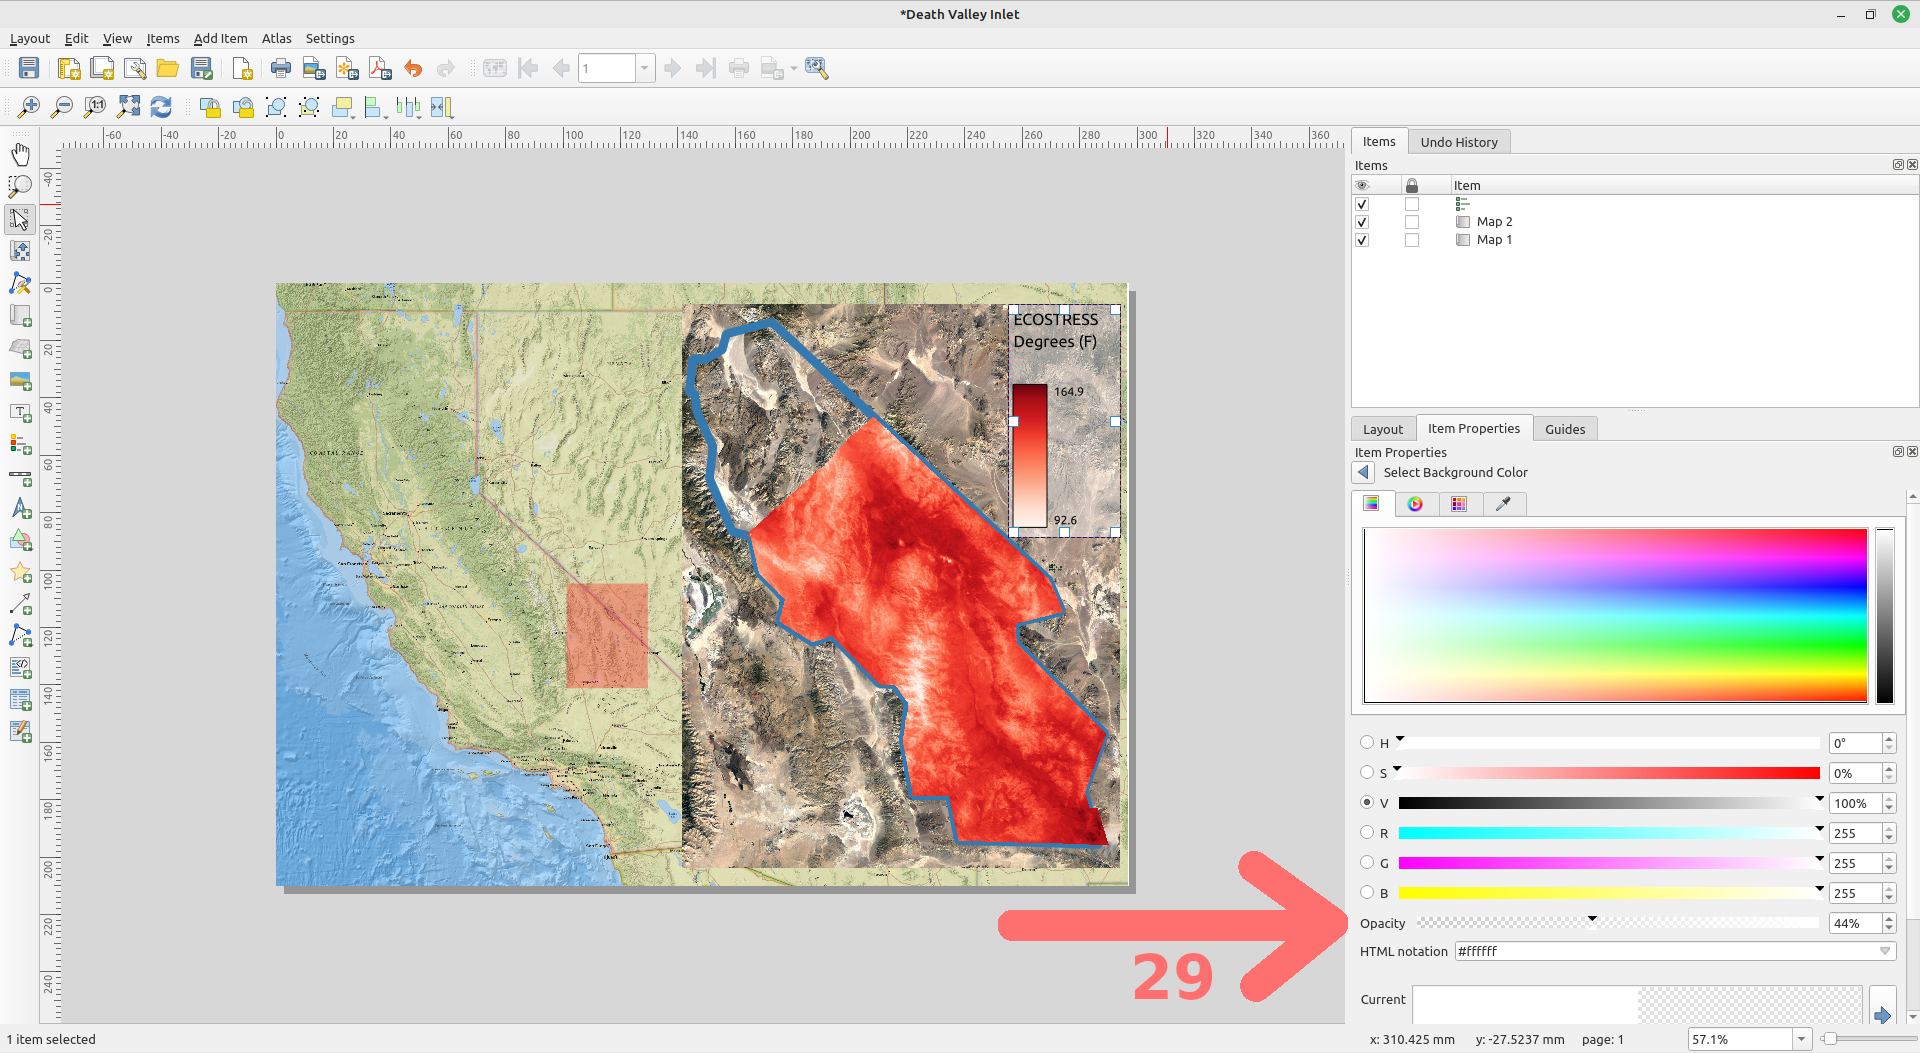
\includegraphics[width=\textwidth]{TempLegend2.png}}


\subsection{Adding Gridlines}

\centerline{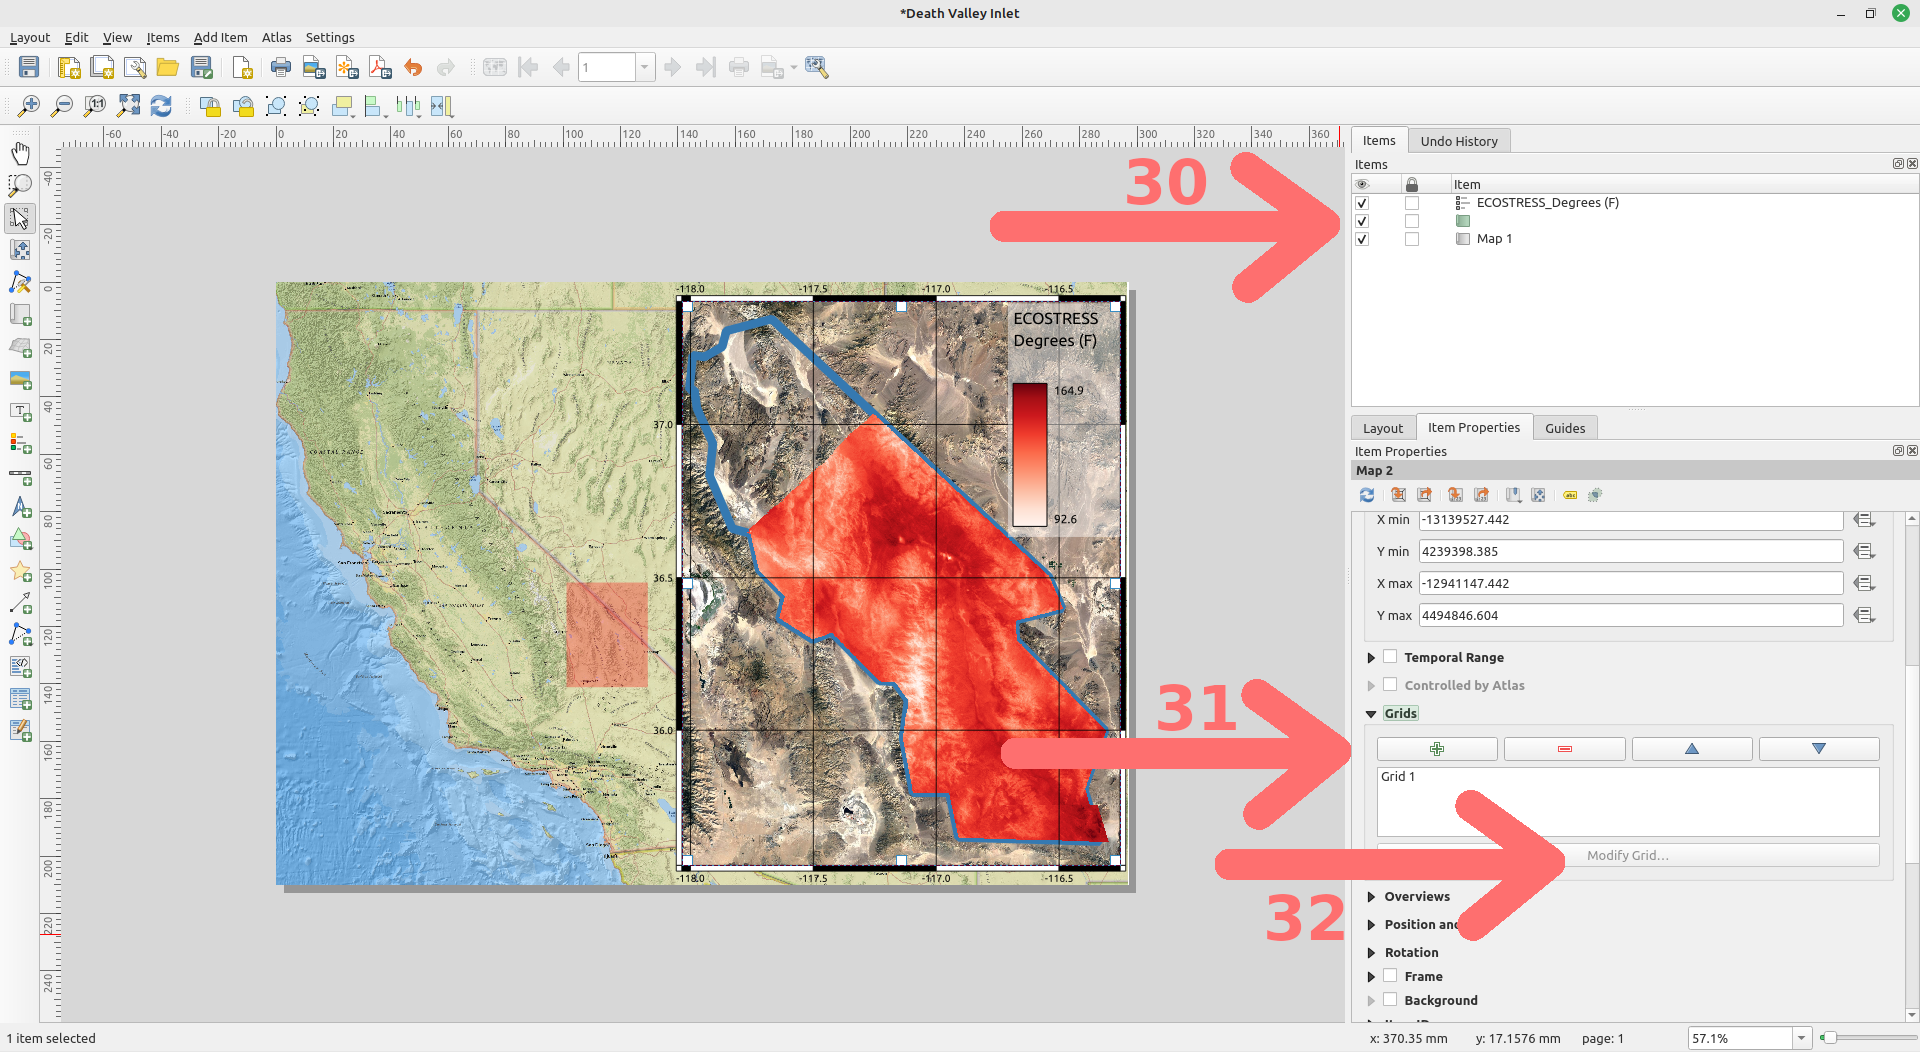
\includegraphics[width=\textwidth]{AddGrid.png}}

30. Let's add gridlines to our inset map so readers can tell where the GPS coordinates of our analyses are at a quick glance. Select the inset map in the \textit{Items} browser, it is likely named "Map 2".

31. Select the \textit{Item Properties} tab and scroll down until you reach the \textit{Grids} subsection. Click the plus sign to add a set of gridlines. By default, the gridlines use the same units and projections as the currently selected map projections. However, it is more common and useful to display grid lines in degrees of latitude and longitude . 

\begin{tcolorbox}[colback=yellow!5!white,colframe=IceCreamLeaf,title=Coordinate Reference Systems (CRS)]
\textbf{Map projections} try to portray the surface of the earth, or a portion of the earth, on a flat piece of paper or computer screen. Essentially, map projections try to transform the earth from its spherical shape (3D) to a planar shape (2D).

A \textbf{coordinate reference system (CRS)} then defines how the two-dimensional, projected map in your GIS relates to real places on the earth. The decision of which map projection and CRS to use depends on the regional extent of the area you want to work in, on the analysis you want to do, and often on the availability of data.
\end{tcolorbox}

32. We can select a different grid \href{https://en.wikipedia.org/wiki/Spatial_reference_system}{coordinate reference system (CRS)} and customize the aesthetics by clicking the \textit{Modify Grid} button.

\vspace{.25em}

\centerline{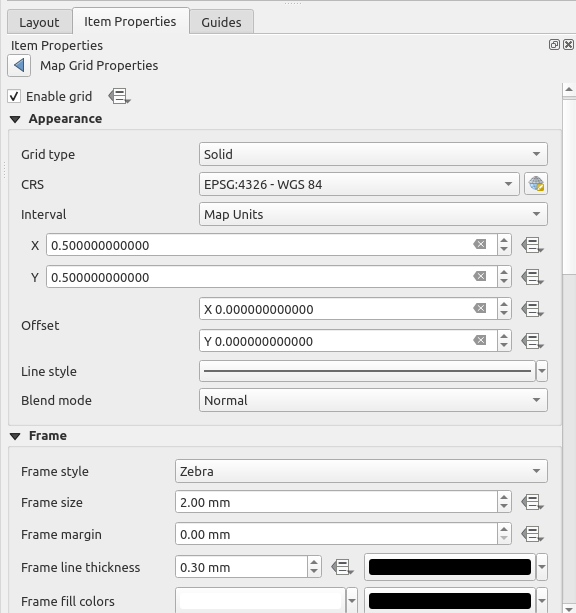
\includegraphics[width=.5\textwidth]{GridProps1.png}}

\begin{singlespacing}
33. Make the following modifications (see above and below screenshots for reference):
	\begin{itemize}
		\item Keep the \textit{Grid Type} as \textit{Solid}. 
		\item Change the \textit{CRS} to \textit{EPSG:4326 - WGS 84} to display GPS coordinates as decimal degrees. 
		\item Change the \textit{X} \& \textit{Y Interval}s to 0.5 to change the spacing of the gridlines.
		\item Change \textit{Frame style} to \textit{Zebra}, because it is a fun style.
		\item Check the box for \textit{Draw Coordinates}.
		\item Disable the \textit{Right} Coordinates because our inset is against the right side of the map.
		\item Change \textit{Coordinate precision} to 1. 
	\end{itemize}
\end{singlespacing}

\centerline{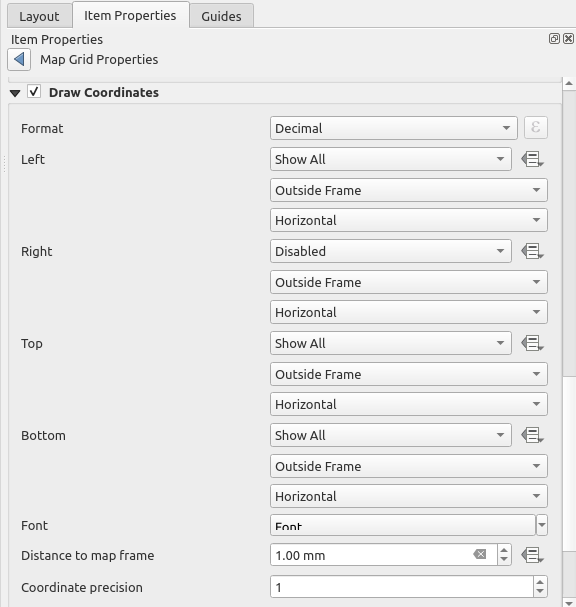
\includegraphics[width=.5\textwidth]{GridProps2.png}}

Your map should now resemble:

\centerline{\includegraphics[width=\textwidth]{DVwGrids.png}}

\kulbox{\textbf{NOTE:} This same procedure could have been done for the main map instead of the inlet map, if that suits your vision.}

Let's add a couple more small details to bring this map to the next level.

\subsection{Adding a Scalebar}

While we now have coordinates for the inset map, it is important for the reader to know the scale of the maps. This is achieved with a scalebar, which QGIS can automatically render for you.

34. With the main map (likely "Map 1") highlighted in the *Items* browser,  click the *Add Item* menu at the top of the screen and select \textit{Add Scalebar}.

35. Draw the scalebar on the main map in a logical place. I like the bottom left corner, which thus far has remained underutilized. 

36. Under \textit{Item Properties} verify that the main map is the map associated with the scalebar. Here you could also adjust the style or units to your liking, but I am just going to stick with the defaults.

\centerline{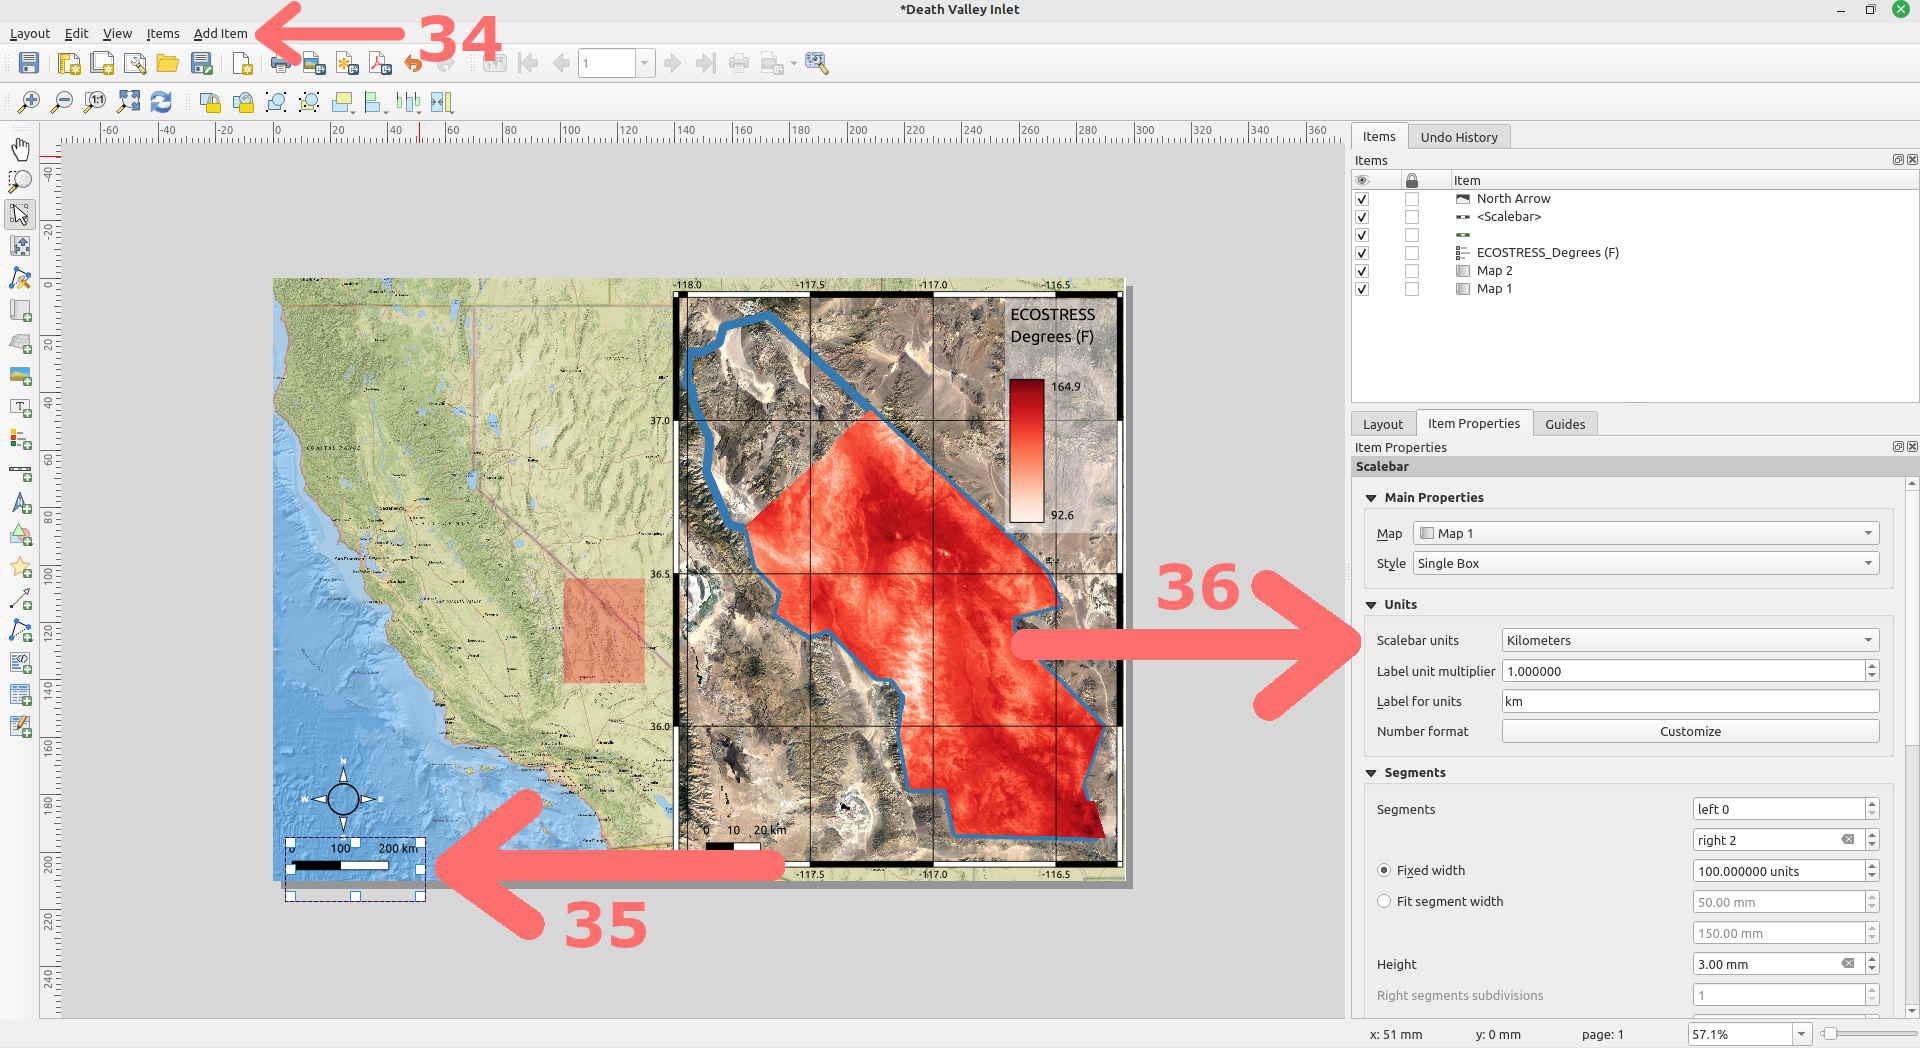
\includegraphics[width=\textwidth]{Scalebar.png}}

\clearpage

\subsection{Adding a North Arrow}

It is customary to indicate which direction is North on a map with a symbol of an arrow pointed North. 

\vspace{.25em}

\centerline{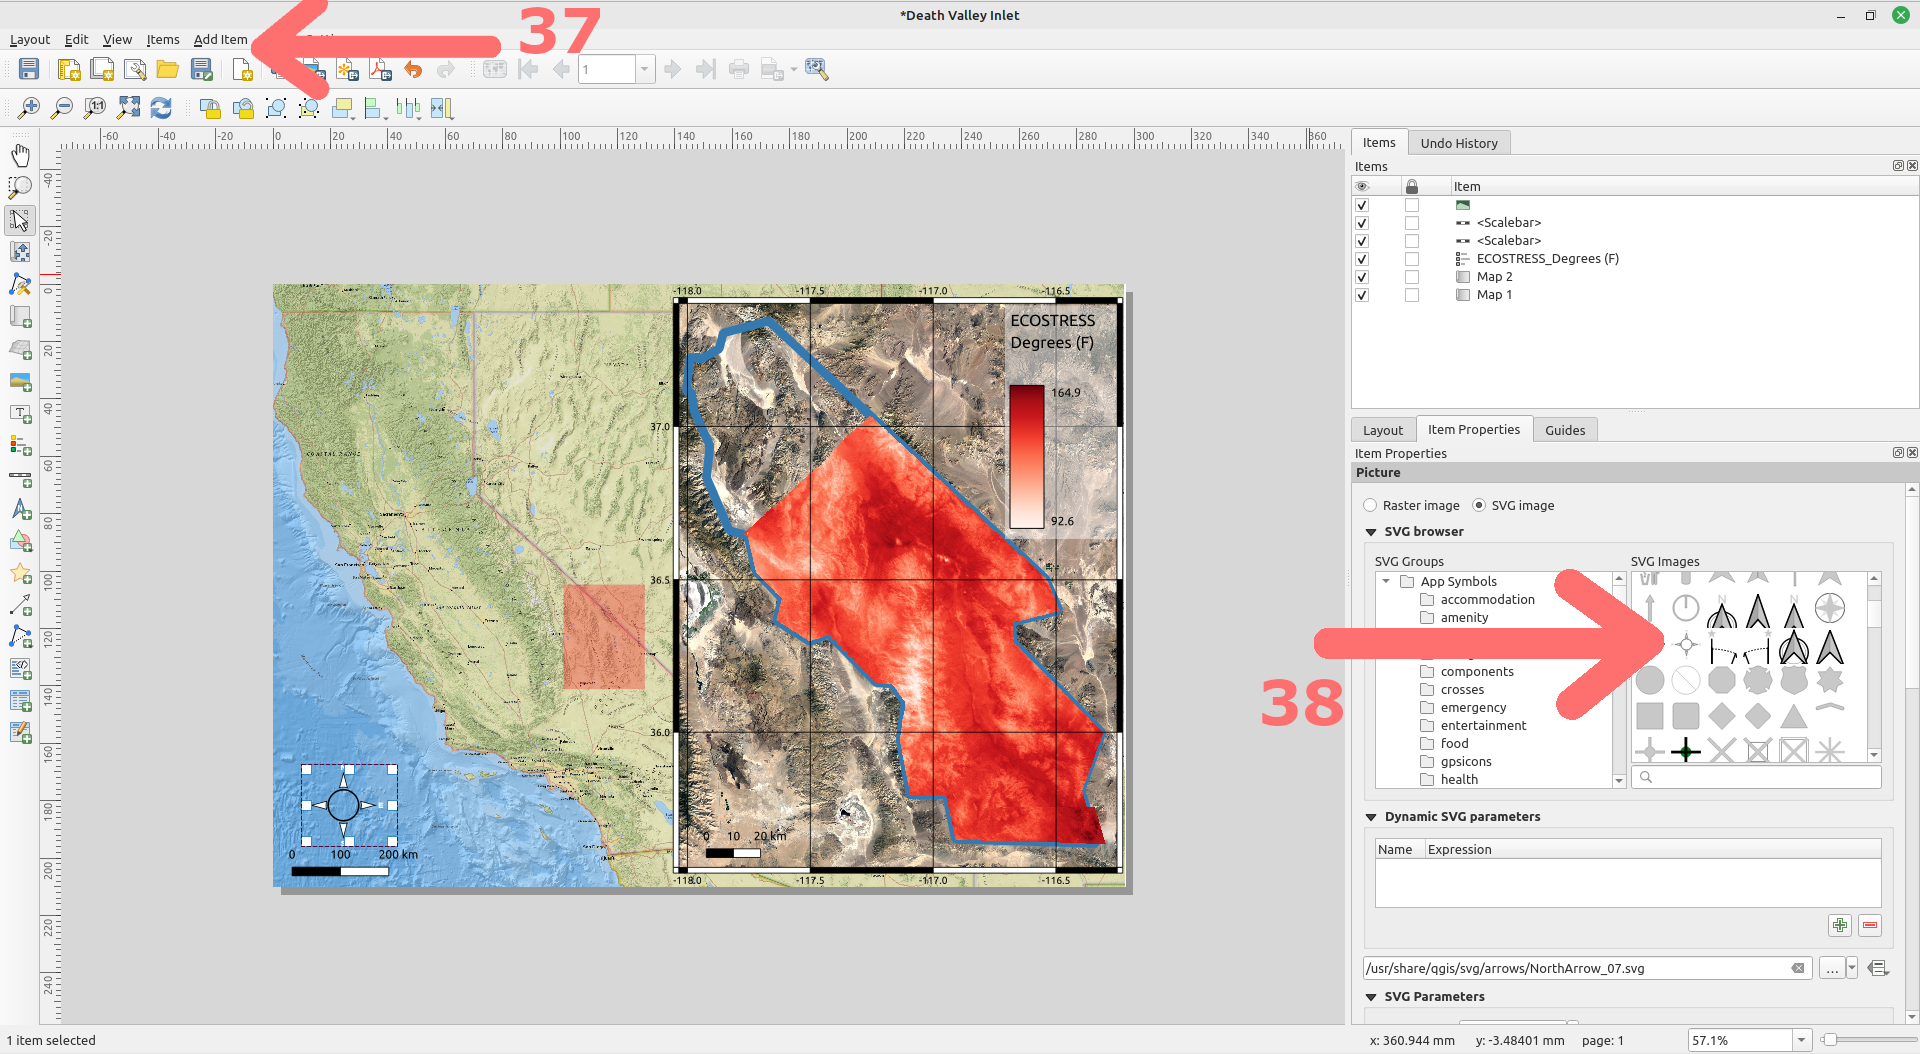
\includegraphics[width=\textwidth]{NorthArrow1.png}}

37. Click the \textit{Add Item} menu at the top of the screen and select \textit{Add North Arrow}.

38. Select your preferred North arrow symbol. I am going with a traditional looking compass style with the cardinal directions labeled. Draw the North arrow in an appropriate place; I selected a centered location above the scalebar. 

\kulbox{\textbf{NOTE:} \textit{SVG Images} tend to look cleaner and sharper compared to the Raster Image options because of the way they store information. Raster files are images built from pixels — tiny color squares that, in great quantity, can form highly detailed images such as photographs. The more pixels an image has, the higher quality it will be, and vice versa. Vector files use mathematical equations, lines, and curves with fixed points on a grid to produce an image. There are no pixels in a vector file. A vector file’s mathematical formulas capture shape, border, and fill color to build an image. Because the mathematical formula recalibrates to any size, you can scale a vector image up or down without impacting its quality. }

\centerline{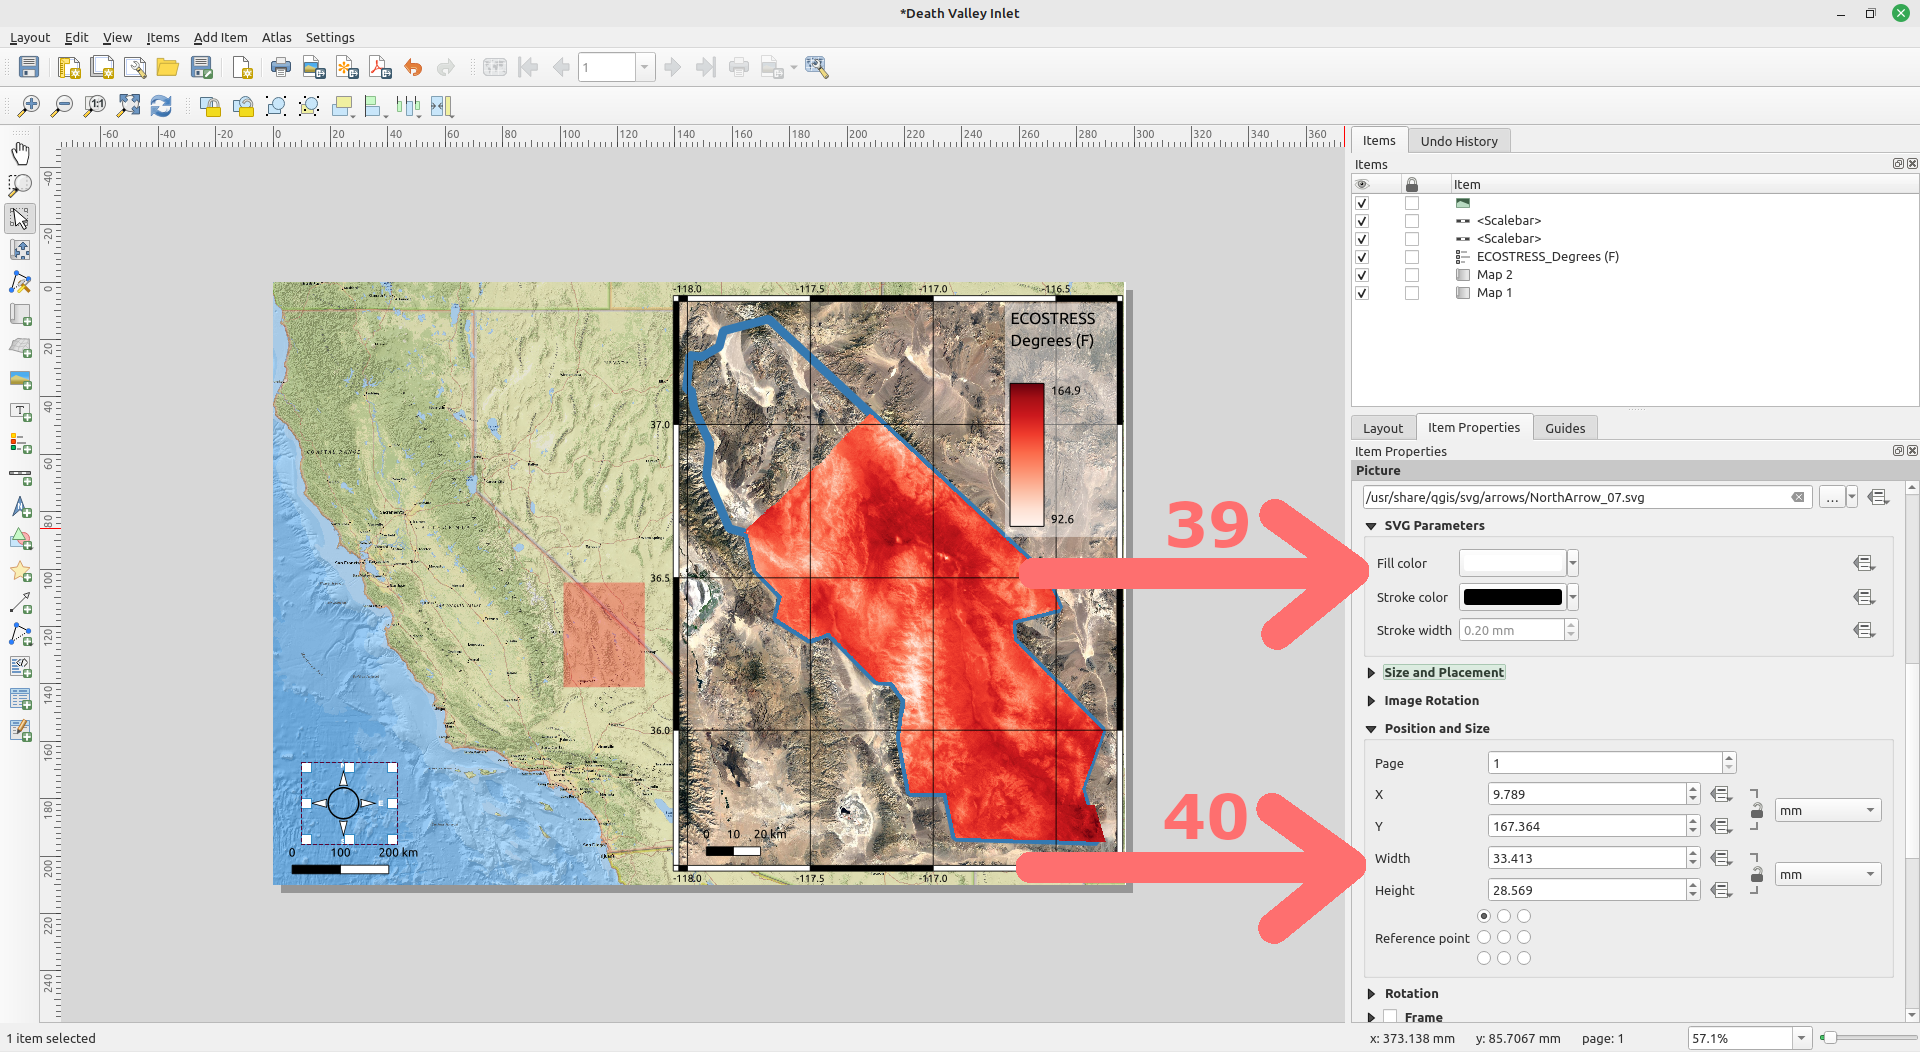
\includegraphics[width=\textwidth]{NorthArrow2.png}}

39.  To adjust the properties of the North arrow, scroll down on the \textit{Item Properties} window to find useful features such as changing color or size.

\subsection{Adding a Title}

\centerline{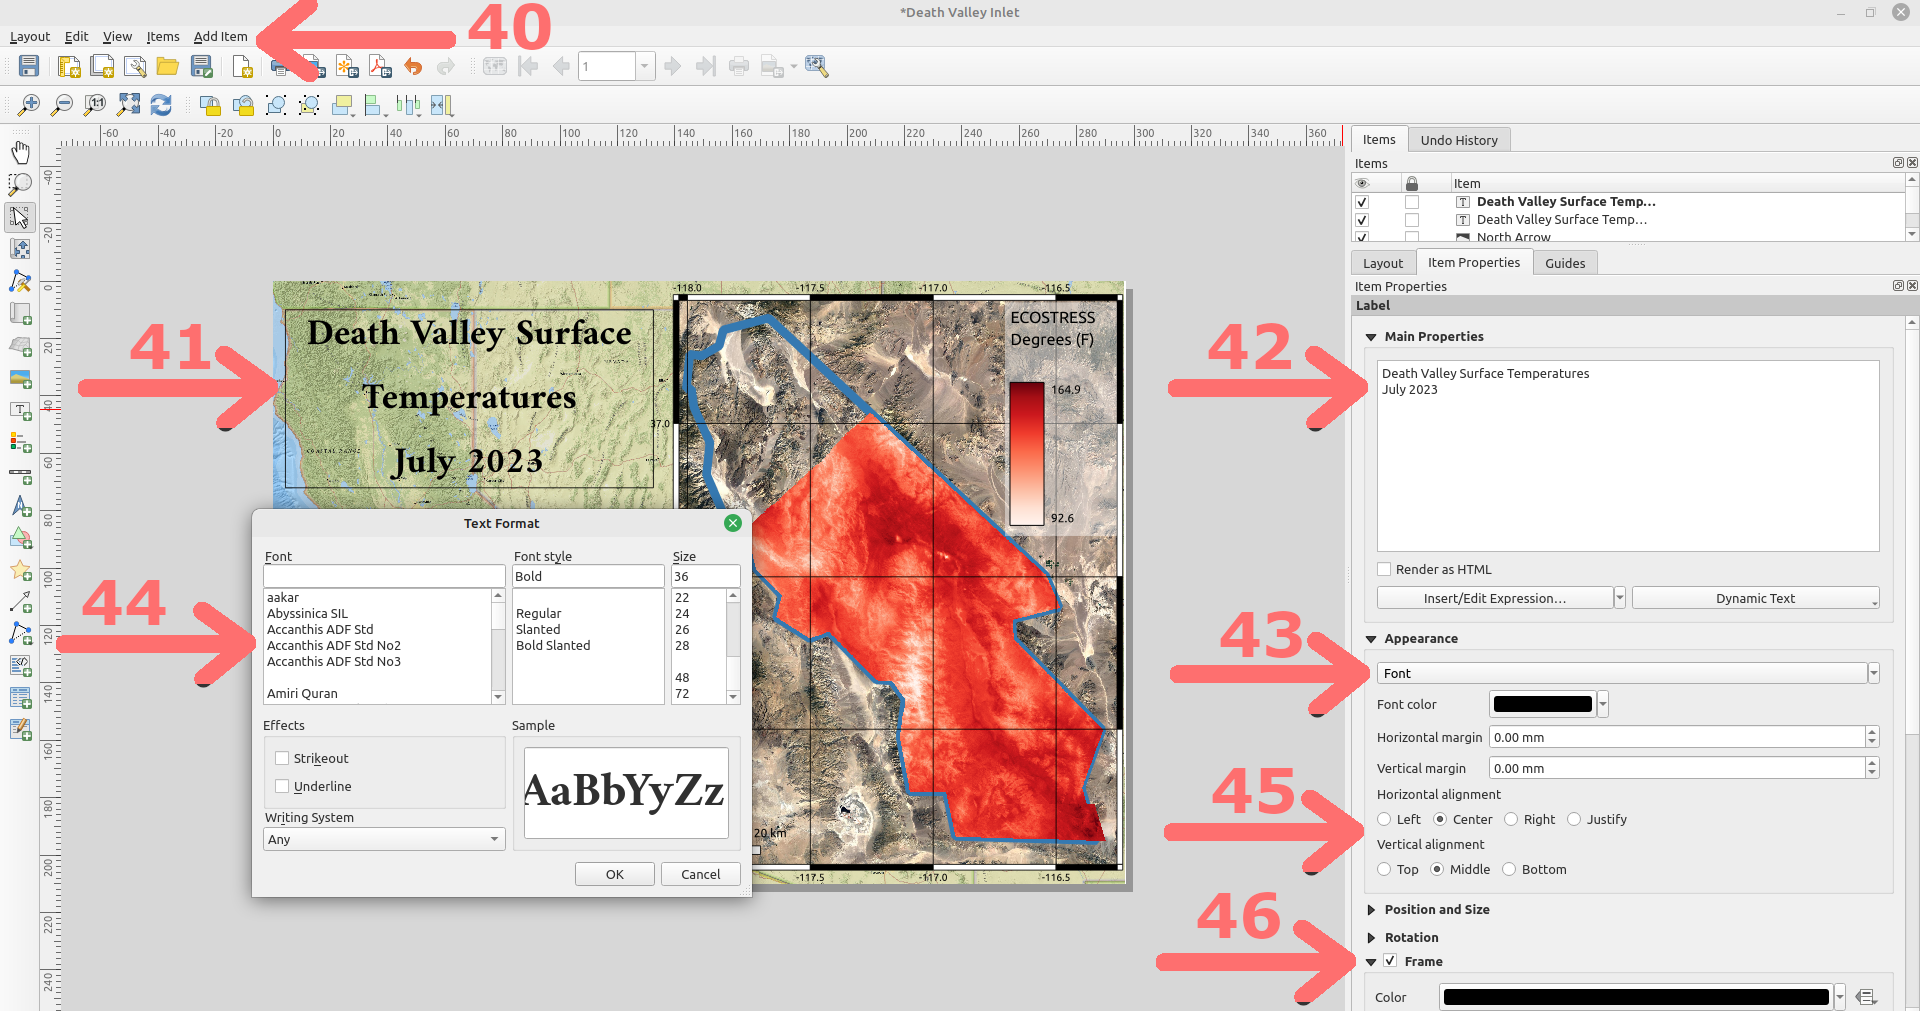
\includegraphics[width=\textwidth]{TextBox.png}}

One last addition, let's add a title to the map to orient the reader to what they are looking at. 

40. Click the \textit{Add Item} menu at the top of the screen and select \textit{Add Label}.

41. Click on your map and draw a box where you want the title to be located. 

42. In the Item Properties tab, expand the Label section and enter the text to title the map, I went with "Death Valley Surface Temperatures - July 2023." 

43. You may want to play around with the spacing to get it to look clean and professional. Under the \textit{Appearance} drop down you can click on the font box to open up the \textit{Text Format} window. 

44. In the {Text Format} window, you can also pick your favorite font and size. You can also change the font color under the \textit{Appearance} dropdown.

45.  You can also adjust the alignment, I set mine to \textit{Center} horizontal alignment and \textit{Middle} vertical.

46. Check the box next to \textit{Frame} and adjust the parameters to draw a frame around your title.

\section{Exporting Your Map}

\centerline{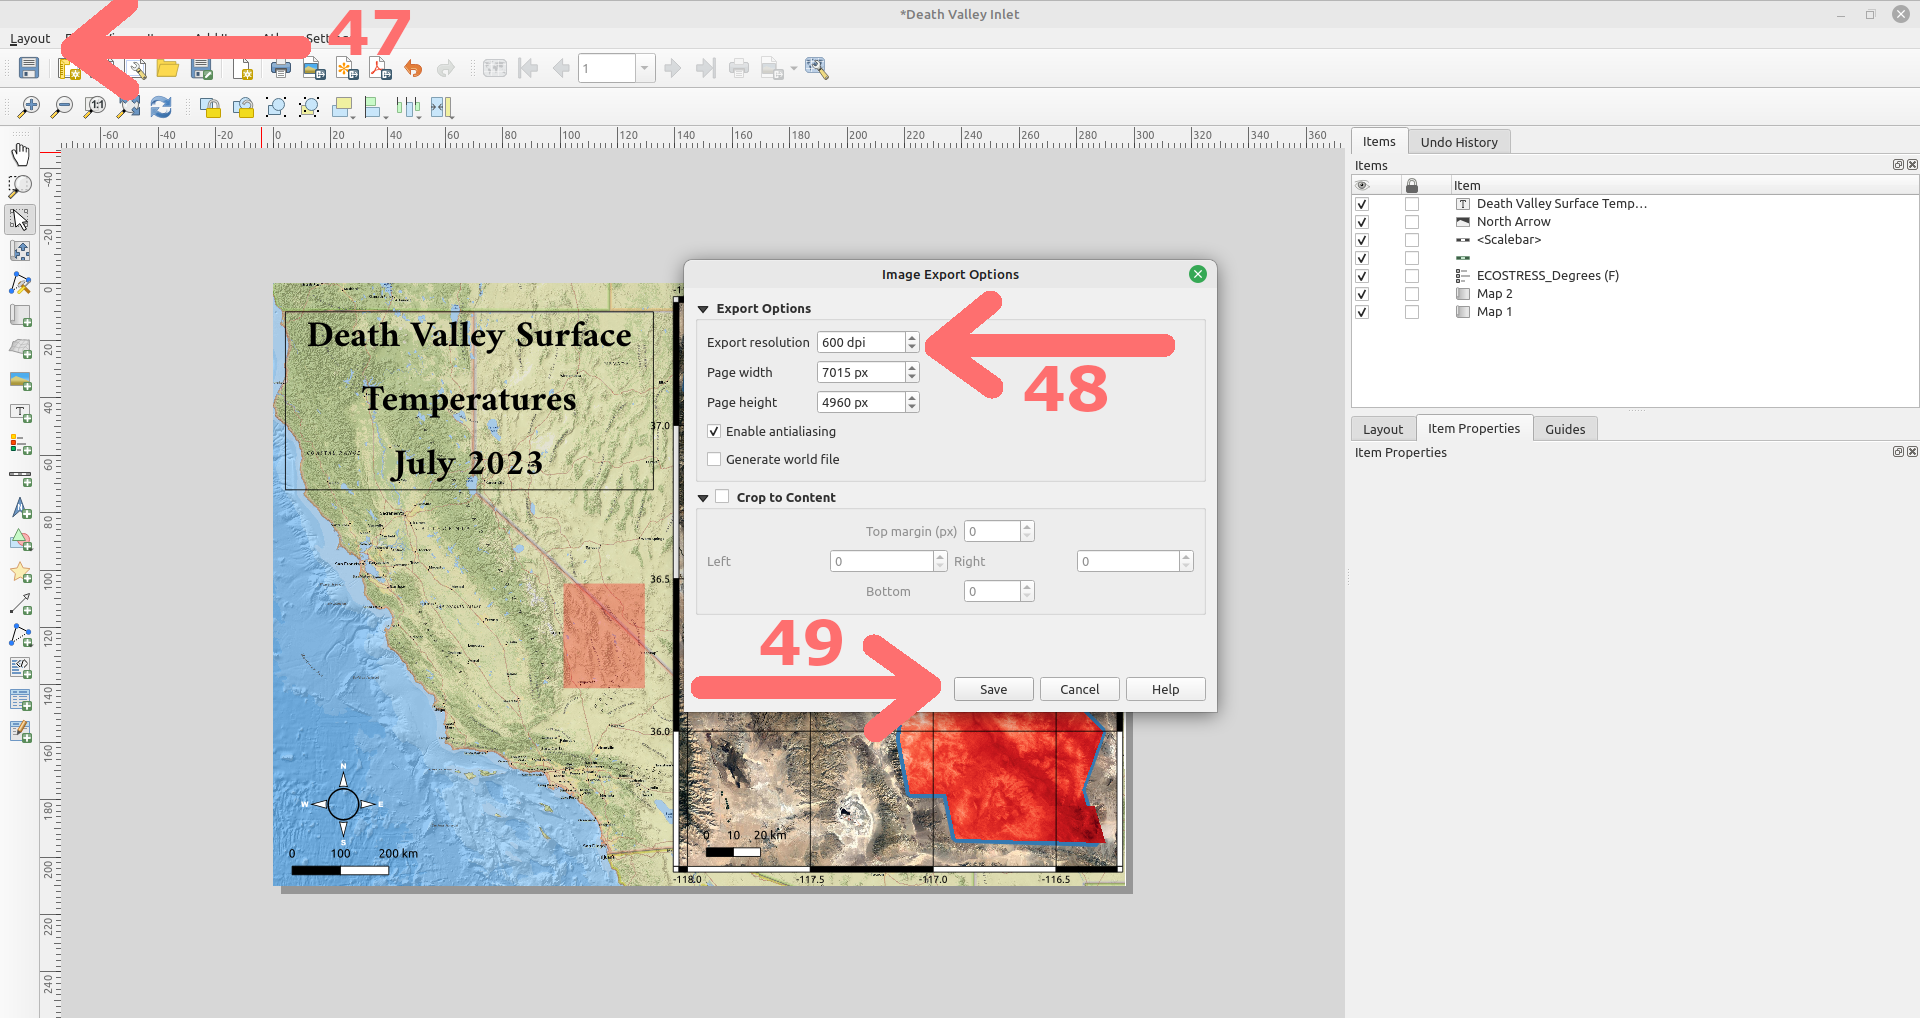
\includegraphics[width=\textwidth]{Export.png}}

Now that our map looks exactly how we want it to look, we want to be able to share it.

47. To do so, select the \textit{Layout} dropdown menu, then \textit{Export as Image}. 

48. The \textit{Export resolution} controls how much detail the output image contains. Smaller resolution $=$ smaller filesize, but with less detail saved. More resolution $=$ more detail saved, but larger filesize. If storage is an issue for you, go with 100 dpi. Otherwise, 300 dpi will generally capture the detail in most cases.

49. Click \textit{Save} and bask in the glory of your first ECOSTRESS map, which (hopefully) resembles the one below. Congratulations...you did a thing!

\kulbox{\textbf{NOTE:} There may be times when you want to export as PDF, particularly when the map needs to be scalable to different sizes.}

\centerline{\includegraphics[width=.75\textwidth]{DeathValleyLSTfinal.png}}

\vspace{.25em}

\hrule

\section{Answering Our Original Question}

\centerline{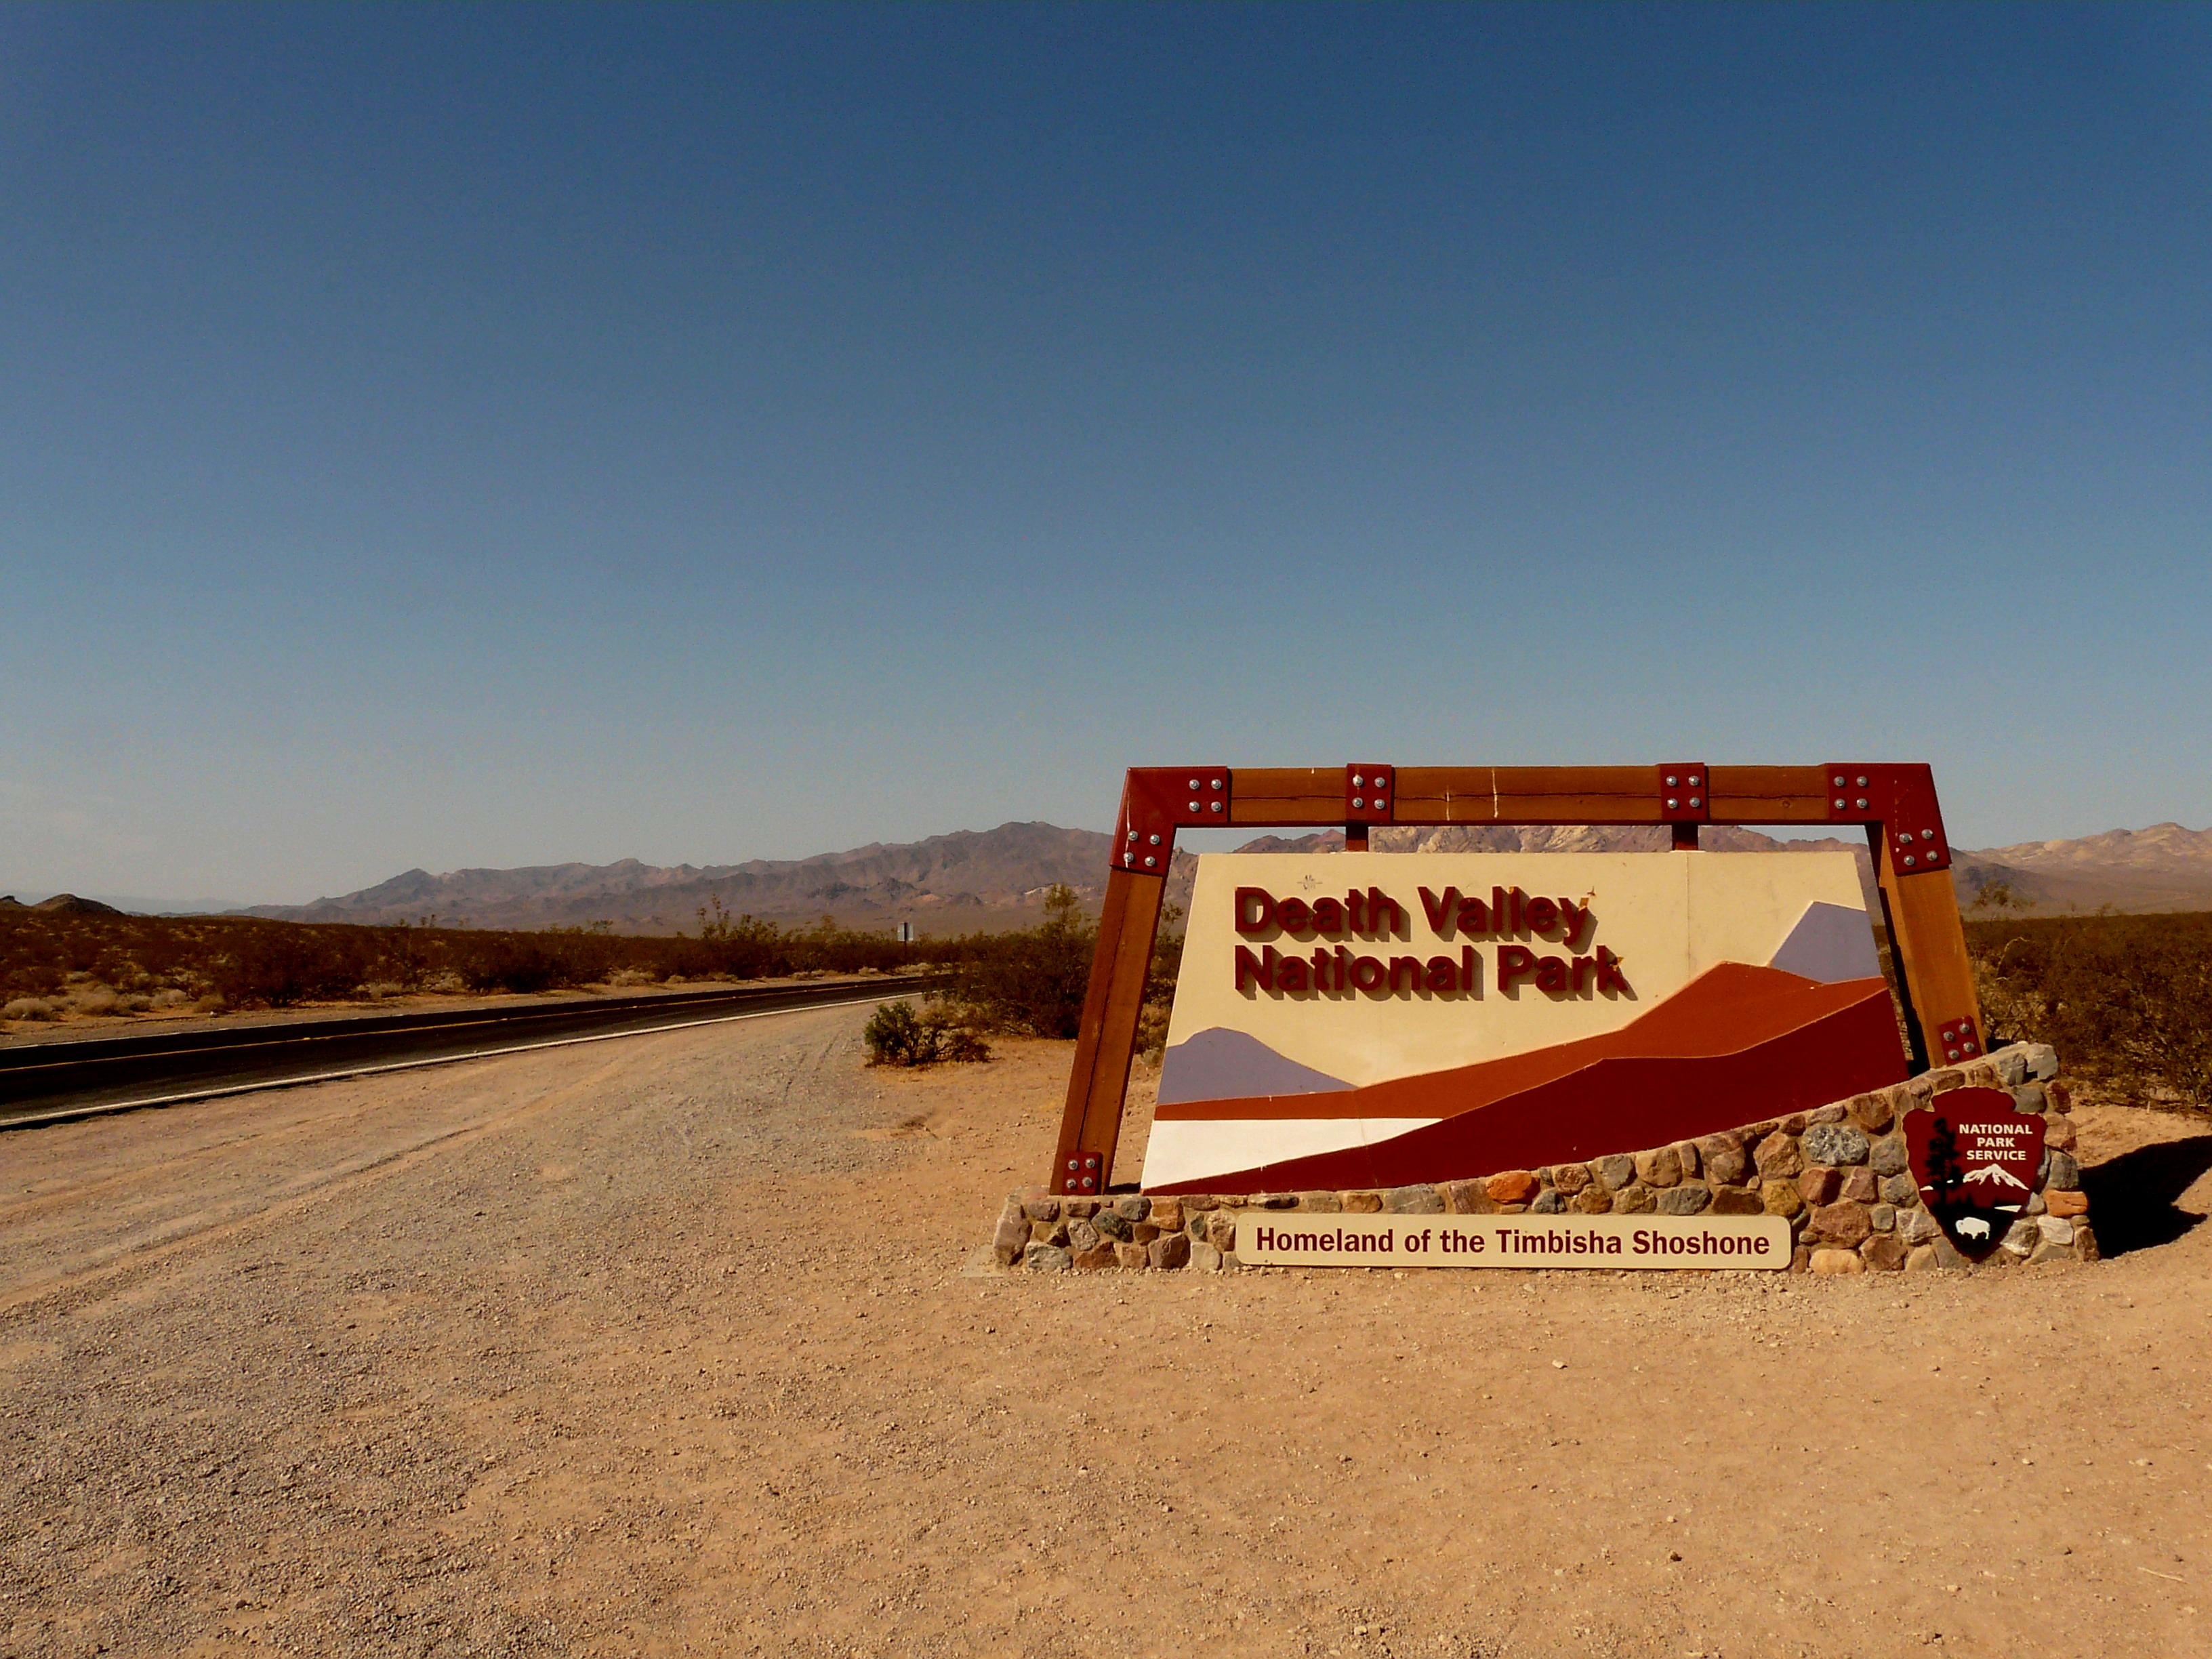
\includegraphics[width=.75\textwidth]{DeathValleySign.jpg}}

If you recall our motivation for this exercise was to see if an analysis with ECOSTRESS supported that land surface temperatures in Death Valley National Park came close to breaking the surface temperature record. 

The highest recorded ground temperature of 201 $^{\circ}$ F was verified on July 15, 1972. It appears that our analysis does not support exceeding that temperature in July 2023, despite that it was one of the hottest months in recorded history for air temperatures. 

\kulbox{\textbf{NOTE:} It is important to remember that the process of science ``supports'' or ``does not support'' hypotheses. It does not ``prove'' or ``disprove'' ideas. There are many factors that prevent our analyses from being entirely conclusive. These include the measurement error of our instruments, the times of day the International Space Station passed over the study site, cloudiness, etc.}

The real power of the ECOSTRESS satellite comes in its geographic and temporal continuity. For instance, it is easy to see from our map which parts of Death Valley have the highest surface temperature. We could also track this seasonally, to see how vegetation growth alters temperatures. The possibilities are endless.

\section{Hometown Temperature Competition Progress}

In the last tutorial (\href{https://jeremydforsythe.github.io/icecream-tutorials/Tutorial4_TemperatureCompetition/Tutorial4_TemperatureCompetition.pdf}{Tutorial \#4: Hometown Temperature Competition}) you learned how to draw a shapefile. Your assignment before today's tutorial was to create a shapefile of your hometown, favorite place you have lived, or somewhere you wish to move in the future and use that file in A$\rho\rho$EEARS to download ECOSTRESS land surface temperature data for last year. Then you were to save GeoTIFF files to your computer of the hottest and coldest land surface temperature observations of that year for your hometown.

\begin{tcolorbox}[colback=yellow!5!white,colframe=IceCreamLeaf,title=\textbf{Temperature Competition Next Steps}]
	Now that you have that data let's put it all together in a map.
	\begin{enumerate}
		\item Start a new project and load the shapefile for your hometown, favorite place you have lived, or somewhere you wish to move in the future.
		\item Use the same procedure we followed in this tutorial to create a map with two insets, one for the hottest and coldest days from the last full calendar year using the GeoTIFF files you saved from the previous tutorial. I have included an example on the next page that I made for Vancouver Island in 2022 for inspiration. You already have all of the skills to make this map! You don't have to make one that exactly mimics the example, but it needs to include all of the design elements that make an effective map: north arrow(s), scalebar(s), title(s), and legend(s). Be creative and curious by exploring the menu options and design a beautiful map that clearly communicates the hottest and coldest temperatures while showcasing your individual style.
	\end{enumerate}
\end{tcolorbox}

\begin{tcolorbox}[colback=yellow!5!white,colframe=IceCreamOrbit,title= \vspace{.2em} \Large Map of the Week Assignments]
	\addcontentsline{toc}{section}{Map of the Week Assignments}
	\large
	\begin{enumerate}
		\item Make a temperature map for your hometown designed to communicate the hottest and coldest temperatures for the last calendar year complete with scalebars(s), north arrow(s), legend(s), title(s), and label(s). 
        \item Provide a one paragraph description of your map. Think of it as an expanded caption. What do you want the reader to know after they see your map? What are the values for the max and min? Are there hotspots or coldspots, and if so why?
	\end{enumerate}
	Submit these assignments via Canvas before Monday's class.
\end{tcolorbox}


\centerline{\includegraphics[width=\textwidth]{Vancouver Island Temperature Competition Example.png}}

\begin{tcolorbox}[colback=yellow!5!white,title=\textbf{Datafiles}]
	\addcontentsline{toc}{section}{Datafiles}
	\large
	In case you encountered any issues with the A$\rho\rho$EEARS database, here are copies of the ECOSTRESS GeoTIFF files for Death Valley:
	\begin{enumerate}
		\item \href{https://jeremydforsythe.github.io/icecream-tutorials/Tutorial2_AccessingRemoteSensingDataWithAppears/ECO2LSTE.001_SDS_LST_doy2023209214149_aid0001.tif}{ECO2LSTE.001\_SDS\_LST\_doy2023209214149\_aid0001.tif}
		\item \href{https://jeremydforsythe.github.io/icecream-tutorials/Tutorial2_AccessingRemoteSensingDataWithAppears/ECO2LSTE.001_SDS_LST_doy2023209214057_aid0001.tif}{ECO2LSTE.001\_SDS\_LST\_doy2023209214057\_aid0001.tif}
	\end{enumerate}
	And Vancouver Island:
	\begin{enumerate}
		\item \href{https://jeremydforsythe.github.io/icecream-tutorials/Tutorial5_AddingElementsToMaps/ECO2LSTE.001_SDS_LST_doy2022339225920_aid0001.tif}{ECO2LSTE.001\_SDS\_LST\_doy2022339225920\_aid0001.tif}
		\item \href{https://jeremydforsythe.github.io/icecream-tutorials/Tutorial5_AddingElementsToMaps/ECO2LSTE.001_SDS_LST_doy2022339212245_aid0001.tif}{ECO2LSTE.001\_SDS\_LST\_doy2022339212245\_aid0001.tif}
		\item \href{https://jeremydforsythe.github.io/icecream-tutorials/Tutorial5_AddingElementsToMaps/ECO2LSTE.001_SDS_LST_doy2022208041543_aid0001.tif}{ECO2LSTE.001\_SDS\_LST\_doy2022208041543\_aid0001.tif}
		\item \href{https://jeremydforsythe.github.io/icecream-tutorials/Tutorial5_AddingElementsToMaps/ECO2LSTE.001_SDS_LST_doy2022208010157_aid0001.tif}{ECO2LSTE.001\_SDS\_LST\_doy2022208010157\_aid0001.tif}
	\end{enumerate}
\end{tcolorbox}

%%%%%%%%%%%%%%%%%%%%%%%%%%%%%%%%%%%%%%%%%%%%%%%%%%%%%%%%%%%%%%%%%%%%%%%%%%%%%%%%%%% End of Document
%\vfill

\hrule

\vspace{1em}

\small \textbf{Recommended Citation:} Forsythe, J.D., G.R. Goldsmith, and J.B. Fisher. 2023. Observing Earth from Above Tutorials. Chapman University. \url{https://jeremydforsythe.github.io/icecream-tutorials/}

\vspace{1em}

This work is supported by funding from NASA ECOSTRESS Mission Grant \#80NSSC23K0309 (I.C.E. C.R.E.A.M.: Integrating Communication of ECOSTRESS Into Community Research, Education, Applications, and Media).

\end{document}
